\thispagestyle{toancuabinone}
\pagestyle{toancuabi}
\everymath{\color{toancuabi}}
%\blfootnote{$^1$\color{toancuabi}Đại học Thăng Long.}
\graphicspath{{../toancuabi/pic/}}
\begingroup
\AddToShipoutPicture*{\put(0,616){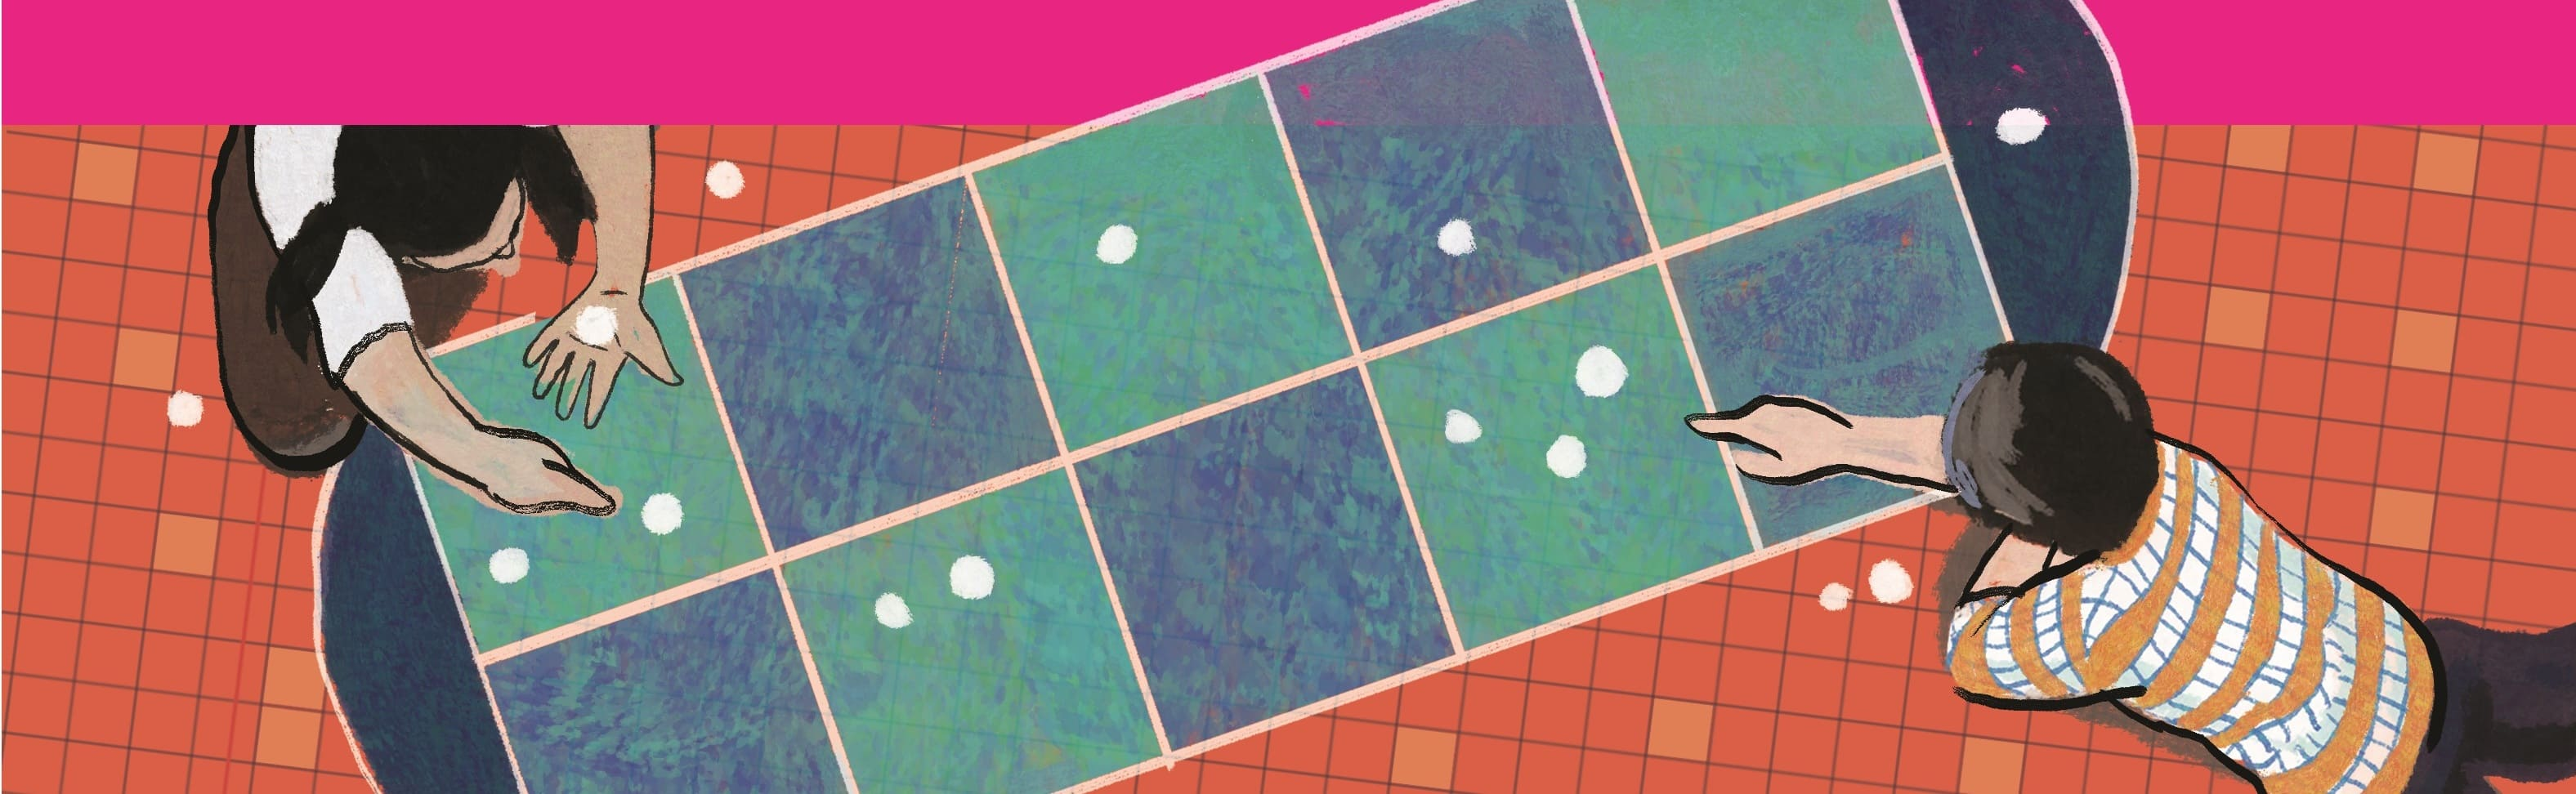
\includegraphics[width=19.3cm]{../bannertoancuabi}}}  
\AddToShipoutPicture*{\put(128,555){
\includegraphics[scale=1]{../tieude1.pdf}}} 
\centering
\endgroup
\vspace*{155pt}

\begin{multicols}{2}
	Trò chơi ``Tháp Hà Nội", xếp những miếng gỗ trên ba chiếc cọc, đã rất quen thuộc với các bạn nhỏ Việt Nam cũng như nhiều bạn nhỏ trên thế giới. Thật là tuyệt vời khi một trò chơi nổi tiếng trên thế giới lại có tên liên quan đến thủ đô của nước ta đúng không. Các bạn đã biết về xuất xứ cùng với nhiều điều thú vị xung quanh bài toán ``Tháp Hà Nội" chưa? Chúng ta hãy cùng ngược dòng thời gian để tìm hiểu qua bài viết dưới đây nhé.
	\vskip 0.1cm
	Năm $1883$, Eduard Lucas (Claus) công bố  bức tranh quảng cáo ``Tháp Hà Nội --  trò chơi thực sự nát óc xứ Annnam":
	\begin{figure}[H]
		\centering
		\vspace*{-5pt}
		\captionsetup{labelformat= empty, justification=centering}
		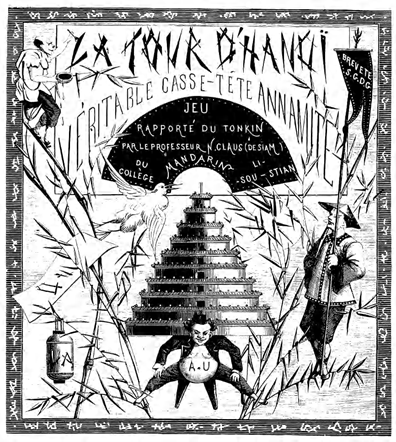
\includegraphics[width=1\linewidth]{1.1}
		%	\caption{\textit{\color{toancuabi}Hình $1$.}}
		\vspace*{-15pt}
	\end{figure}
	Một năm sau, Lucas viết bài ``Tháp Hà Nội , trò chơi toán học" đăng ở tạp chí ``Science et Nature", số $1$ ($1884$) tr. $127-128$. Có thể xem đó ngày khai sinh của ``Bài toán Tháp Hà Nội", một trong những bài toán nổi tiếng của toán học. Cho đến ngày nay, vẫn còn rất nhiều công trình nghiên cứu về bài toán tháp Hà Nội và những mở rộng của nó, vẫn còn nhiều giả thuyết đang chờ câu trả lời.
	\vskip 0.1cm
	Hình sau đây là bức ảnh chụp từ hiện vật trưng bày trong ``Musée des arts et métiers--Cnam Paris" (Bảo tàng nghệ thuật và thủ công Paris). 
	\begin{figure}[H]
		\centering
		\vspace*{-5pt}
		\captionsetup{labelformat= empty, justification=centering}
		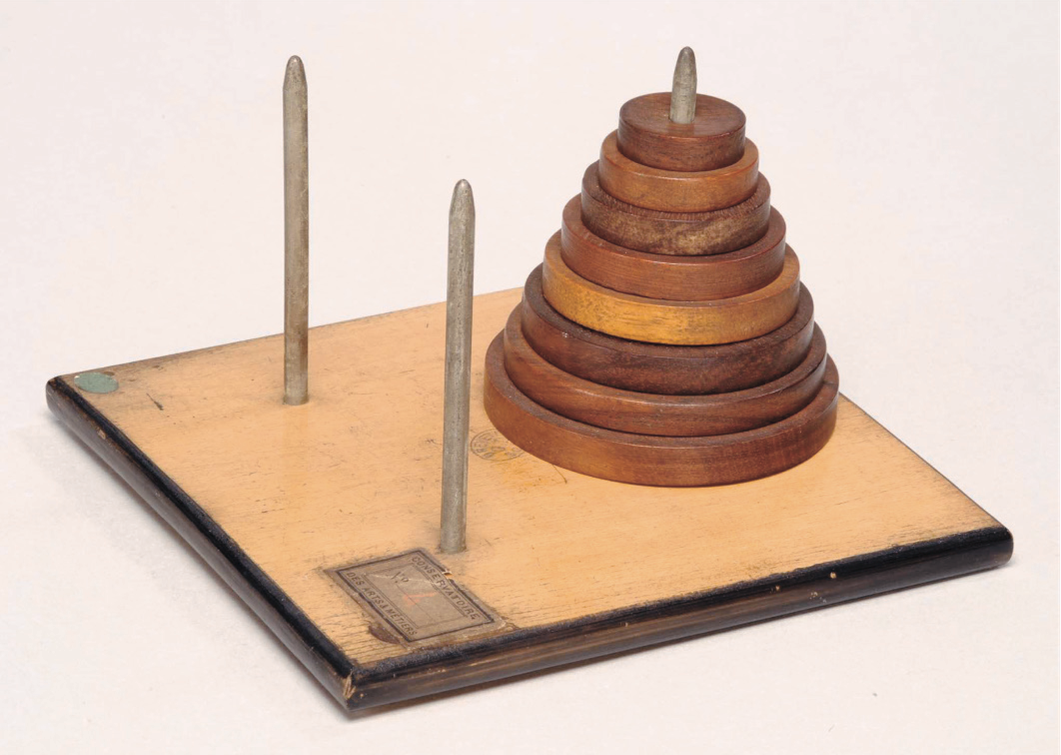
\includegraphics[width=1\linewidth]{2.1}
		%	\caption{\textit{\color{toancuabi}Hình $1$.}}
		\vspace*{-15pt} 
	\end{figure}
	Ta có ba cái cọc, và  $8$ cái đĩa với kích thước khác nhau đôi một. Bài toán đặt ra là di chuyển toàn bộ $8$ cái đĩa sang một cọc khác, sao cho vẫn giữ được thứ tự các đĩa với bán kính lớn dần từ trên xuống dưới. Quy tắc di chuyển: mỗi lần chỉ được chuyển một đĩa, và không bao giờ được đặt một đĩa lên đĩa khác có bán kính nhỏ hơn. Điều này có thể làm được nhờ sử dụng cọc ``trung gian".
	\vskip 0.1cm
	Các bạn thử hình dung xem ta sẽ cần làm bao nhiêu phép chuyển đĩa?
	\vskip 0.1cm
	Trước hết, ta thử làm bài toán dễ hơn: trên cọc chỉ có $2$ đĩa. Rõ ràng chỉ cần chuyển đĩa nhỏ sang cọc trung gian, đĩa lớn sang cọc còn lại, rồi chuyển đĩa nhỏ lên cọc đó. Số bước chuyển là $3$.
	\vskip 0.1cm
	Nếu có $3$ đĩa trên cọc thì sao? Giả sử các đĩa đang ở cọc $A$, và ta cần chuyển sang cọc $C$. Ta chuyển hai đĩa trên cùng sang cọc  trung gian $B$, rồi chuyển đĩa to nhất sang cọc $C$. Sau đó chỉ cần chuyển hai đĩa từ cọc $B$ sang cọc $C$. Phương pháp chuyển $2$ đĩa từ cọc này sang cọc khác thì ta đã biết. Như vậy, số phép chuyển phải làm khi có $3$ đĩa bằng $2$ lần số phép chuyên khi có $2$ đĩa, cộng thêm $1$ phép chuyển (đĩa to nhất). 
	\vskip 0.1cm
	Như vậy, số bước chuyển cần thiết của $3$ đĩa là: $2\times 3 + 1 = 7$. Bằng quy nạp, dễ chứng minh nếu $N$ là số phép chuyển khi có $n$ đĩa thì với $(n+1)$ đĩa, ta có thể thực hiện nhiệm vụ với $(2N+1)$ phép chuyển. Từ đó, dễ suy ra, nhiệm vụ đặt ra trong bài toán Tháp Hà Nội với $n$ đĩa có thể thực hiện với $2^n- 1$  phép chuyển.
	\vskip 0.1cm
	Có thể chứng minh $2^n - 1$  là số phép dịch chuyển tối thiểu cần thiết, nghĩa là không có cách gì thực hiện nhiệm vụ với số phép dịch chuyển ít hơn.
	\vskip 0.1cm
	Người ta cho rằng, bài toán Tháp Hà Nội lấy ý tưởng từ câu chuyển cổ Ấn Độ sau đây.
	\vskip 0.1cm
	``Trong ngôi đền vĩ đại ở Benares, bên dưới mái vòm đánh dấu trung tâm thế giới, người ta đặt một chiếc đĩa bằng đồng, trên đó gắn cố định ba chiếc cọc kim cương, mỗi chiếc cao một mét và dày như thân của một con ong. Trên một trong những chiếc cọc  kim cương đó, vào buổi sáng tạo, Thượng Đế đặt $64$ chiếc đĩa bằng vàng nguyên chất, theo thứ tự to dần từ trên xuống dưới.  Ngày đêm không ngừng, những con quỷ chuyển các đĩa từ cọc kim cương này sang cọc kim cương khác theo nguyên tắc không được di chuyển nhiều hơn một đĩa cùng một lúc, và không được đặt đĩa nào lên trên cái nhỏ hơn nó. Khi $64$ chiếc  đĩa  được chuyển xong thì tiếng sét sẽ nổ ra, và thế giới tan biến".
	\vskip 0.1cm
	Những suy luận trên đây chỉ ra rằng, số phép dịch chuyển mà lũ quỷ phải làm ít nhất là
	\begin{align*}
		2^{64} - 1= 18{.}446{.}744{.}073{.}709{.}551{.}615.
	\end{align*}
	Giả sử lũ quỷ rất thạo ``thuật toán dịch chuyển", và mỗi giây chúng chuyển được một đĩa, thì phải mất khoảng $585$ tỷ năm. Có lẽ dù không có lũ quỷ, trái đất của chúng ta cũng không tồn tại được lâu đến thế!
	\vskip 0.1cm
	Từ sau khi ra đời, bài toán Tháp Hà Nội nhận được sự quan tâm lớn của các nhà toán học và những người làm ... đồ chơi. Rất nhiều phiên bản của bài toán Tháp Hà Nội xuất hiện, chẳng hạn như số cọc lớn hơn $3$, hoặc cách chơi có thay đổi. Cho đến ngày nay, Tháp Hà Nội và những biến thể của nó vẫn là bài toán quan trọng trong toán học rời rạc, lý thuyết đồ thị, khoa học máy tính, và tô pô (chẳng hạn, bài toán về đường cong tự cắt tại mọi điểm của nó!). Thậm chí, Tháp Hà Nội còn có ứng dụng rộng rãi trong nghiên cứu tâm lý học!
	\vskip 0.1cm
	Người ta cho rằng, sở dĩ bài toán Tháp Hà Nội lôi cuốn được nhiều thế hệ các nhà toán học vì nó chứa đựng những yếu tố làm nên sức hấp dẫn của Toán học: đẹp, thú vị, hữu ích, và bất ngờ.
\end{multicols}
\newpage
\begingroup
\AddToShipoutPicture*{\put(78,675){
\includegraphics[scale=1]{../tieude.pdf}}} 
\centering
\endgroup
\vspace*{30pt}

\begin{multicols}{2}
	Thám tử Xuân Phong cùng thanh tra Lê Kính tham gia một buổi giới thiệu sản phẩm của hai công ty là Tae Yeon và TeaYon tại triển lãm Điện tử Expo -- New Vision của khu vực. Công ty  Tae Yeon có uy tín từ lâu đời, với những sản phẩm tinh tế có chất lượng tốt nổi tiếng,  các nhân viên của công ty luôn nói thật. Còn công ty TeaYon chuyên sản xuất đồ rẻ, kém chất lượng, bắt chước kiểu dáng của công ty Tae Yeon nên ban giám đốc dặn các nhân viên của mình chỉ được nói dối trong buổi triển lãm. 
	\vskip 0.1cm
	Vừa đặt chân tới khu vực triển lãm được trang hoàng lộng lẫy, Xuân Phong gặp ngay $5$ đại diện  của hai công ty này đứng tại cổng ra vào và tươi cười niềm nở tiếp đón. Xuân Phong tiến tới họ và hỏi cả $5$ người cùng một câu hỏi ``Có bao nhiêu người đến từ công ty Tae Yeon trong số các bạn?" 
	\vskip 0.1cm
	Người thứ nhất trả lời ``Không có ai cả". Hai người tiếp theo đều trả lời ``Có đúng một người". 
	\vskip 0.1cm
	Vậy hai người còn lại sẽ trả lời câu hỏi của thám tử Xuân Phong như thế nào nhỉ? Em có thể suy đoán ra câu trả lời của họ và giải thích lập luận được không?
	\begin{figure}[H]
		\centering
		\vspace*{-5pt}
		\captionsetup{labelformat= empty, justification=centering}
		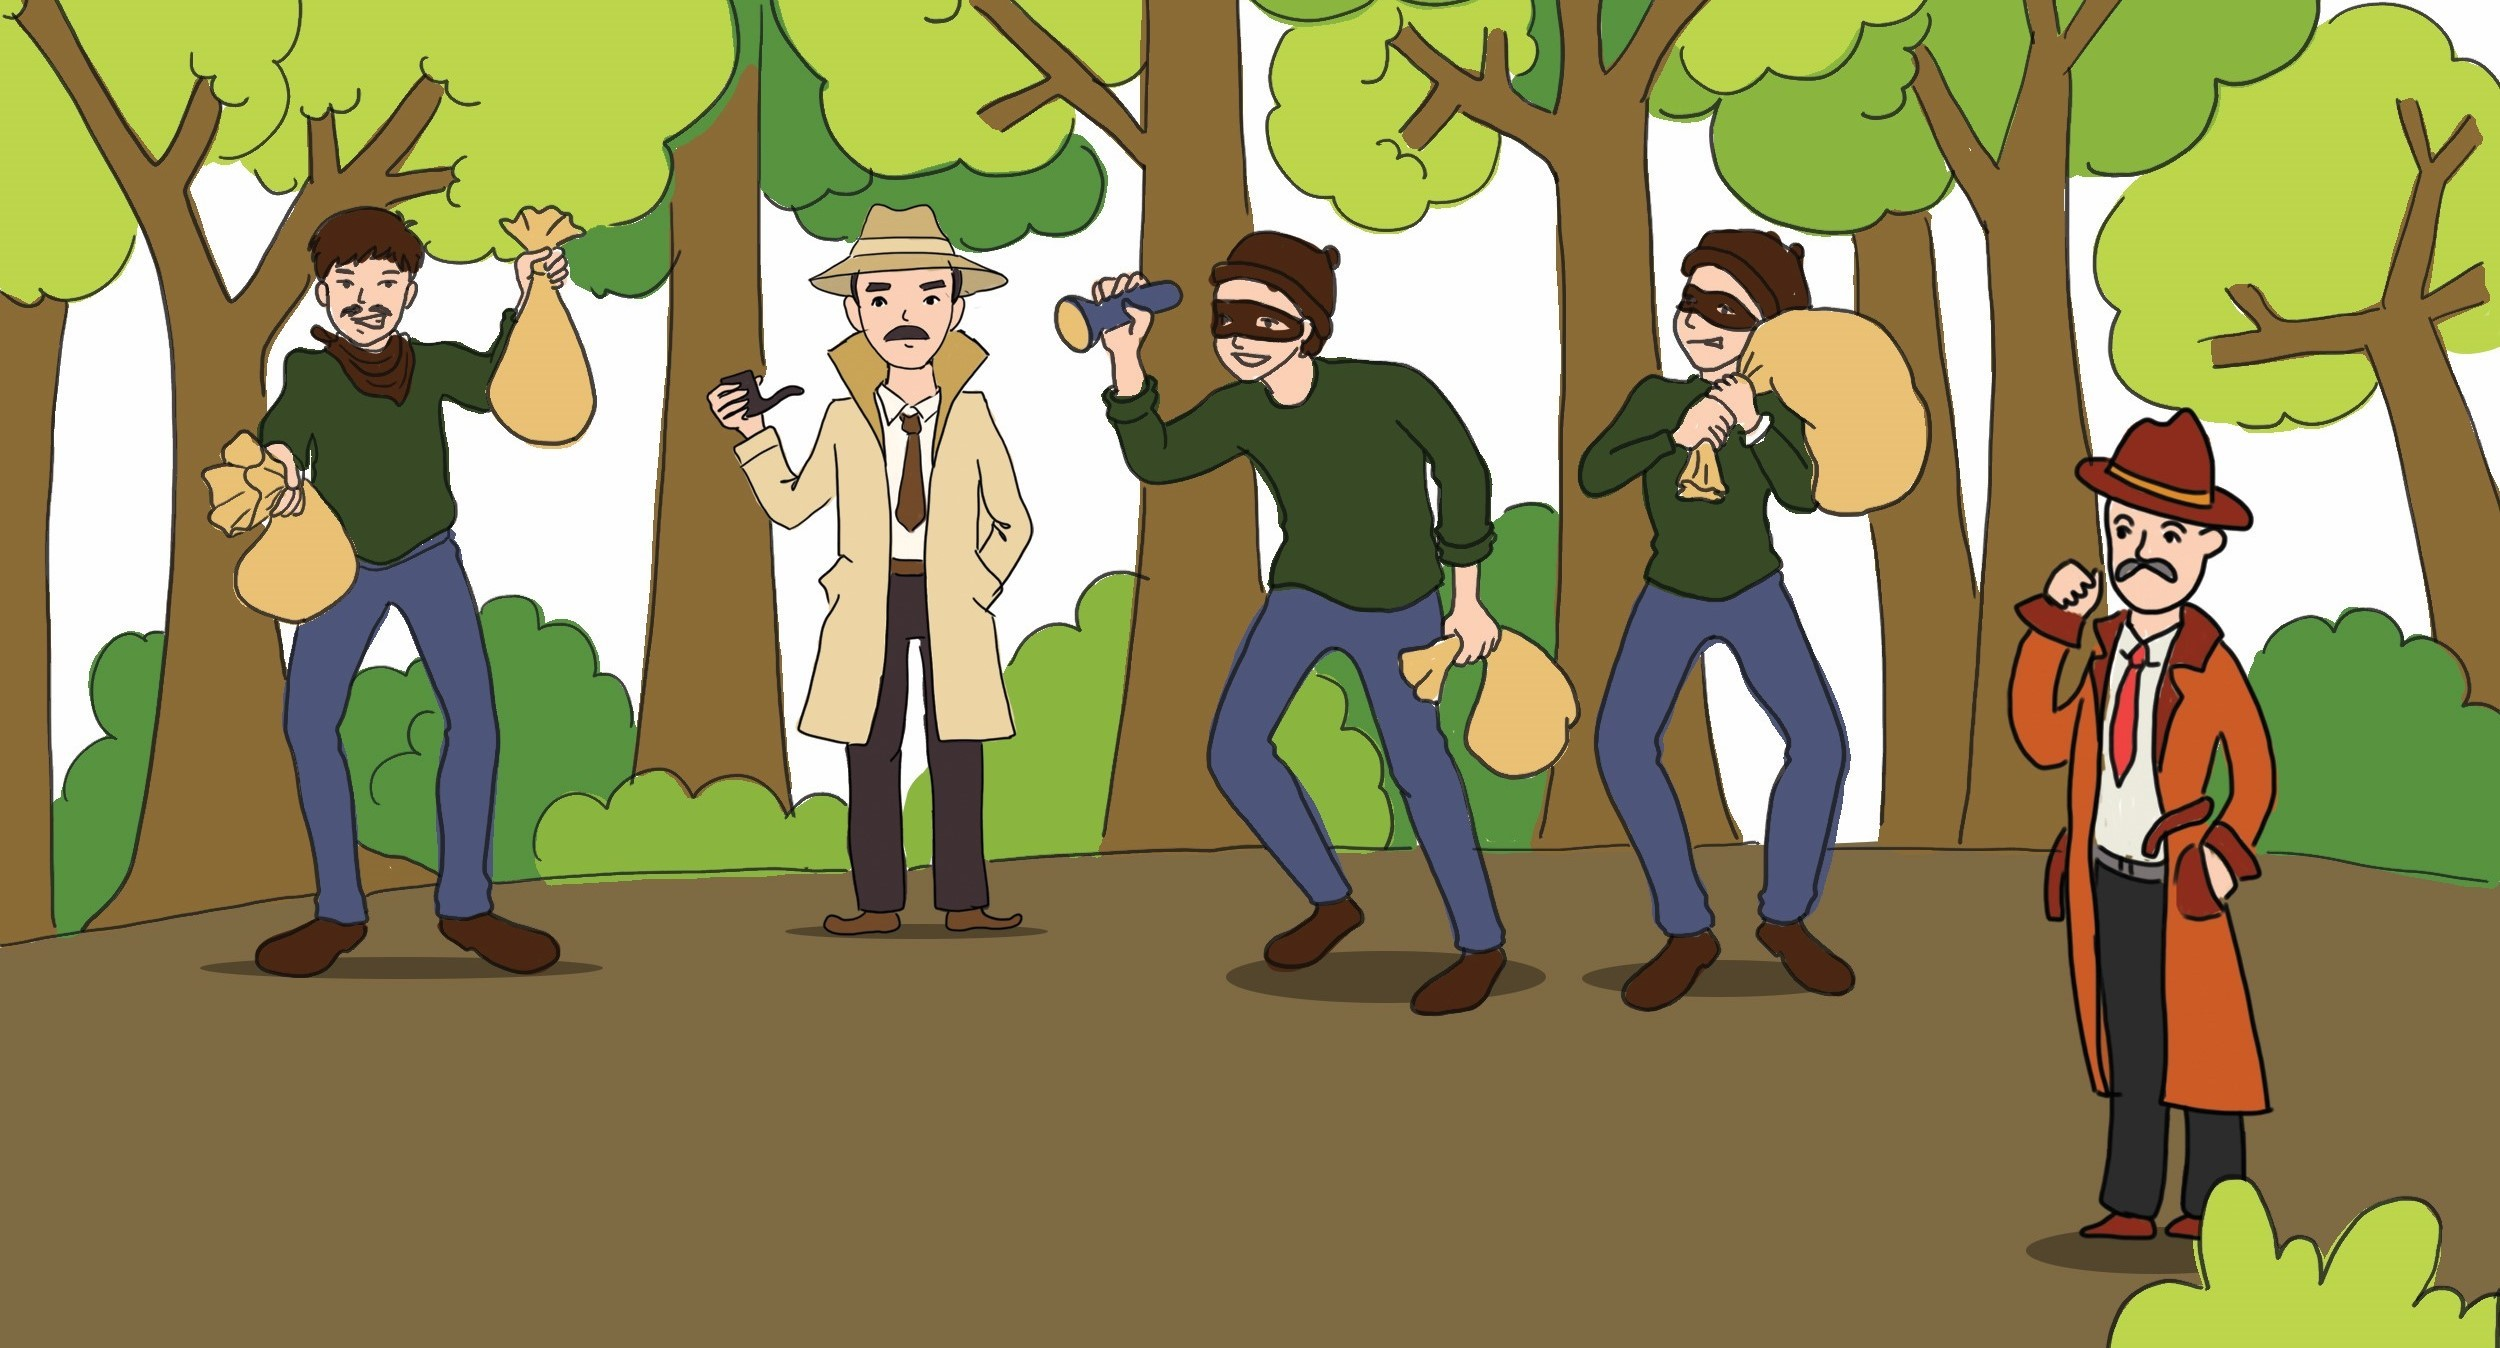
\includegraphics[width=1\linewidth]{xuanphong}
		\vspace*{-5pt}
	\end{figure}
%	
%	Người của công ty Tae Yeon không thể trả lời ``Không có ai cả" vì như vậy người đó sẽ nói dối. Vì vậy, người đầu tiên đến từ công ty TeaYon. 
%	\vskip 0.1cm
%	Hai người tiếp theo trả lời giống nhau, vì thế họ phải cùng nói thật hoặc cùng nói dối, tức là đến từ cùng một công ty.
%	\vskip 0.1cm
%	Nếu cả hai người này cùng đến từ công ty Tae Yeon, suy ra số người của công ty Tae Yeon trong số họ không ít hơn $2$ người. Suy ra câu trả lời của họ là sai. Vì vậy cả hai người thứ hai và thứ ba đều nói dối, tức là đến từ công ty TeaYon.
%	\vskip 0.1cm
%	Do vậy, trong số $5$ người này, có ít nhất $3$ người của công ty TeaYon và không quá $2$ người đến từ công ty Tae Yeon.
%	\vskip 0.1cm
%	Nhưng vì cả $3$ người đầu tiên đều nói dối, suy ra số người của công ty Tae Yeon trong số họ không thể là $0$ hoặc $1$. Vì vậy, cả hai người còn lại đều là nhân viên của công ty Tae Yeon. Và họ đều sẽ trả lời là ``Có hai người".
\end{multicols}
\vspace*{-10pt}
{\color{toancuabi}\rule{1\linewidth}{0.1pt}}
\begingroup
\AddToShipoutPicture*{\put(115,305){
\includegraphics[scale=1]{../tieude11.pdf}}} 
\centering
\endgroup
\vspace*{53pt}

\begin{multicols}{2}
	$\pmb{1.}$	Trong một cuộc thi thể thao, ban tổ chức chọn ra một số bạn học sinh ở lớp $5A$ và một số bạn ở lớp $5B$ thi đấu trực tiếp. Mỗi bạn ở lớp $5A$ được chọn ra sẽ thi đấu duy nhất một trận với một bạn ở lớp $5B$, và ngược lại, mỗi bạn ở lớp $5B$ được chọn ra chỉ đấu đúng một trận với một bạn ở lớp $5A$.
	\begin{figure}[H]
		\centering
		\vspace*{-5pt}
		\captionsetup{labelformat= empty, justification=centering}
		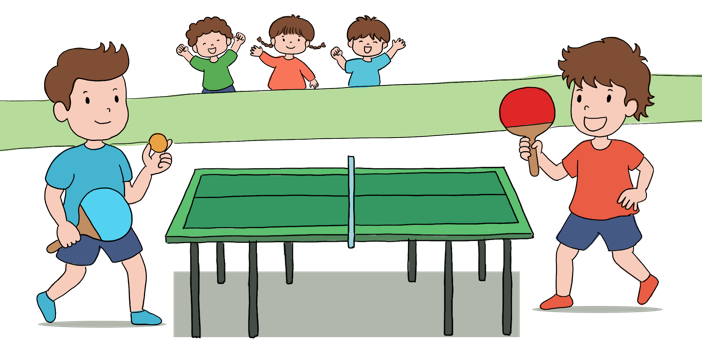
\includegraphics[width=1\linewidth]{Pi5_bai1}
		\vspace*{-15pt}
	\end{figure}
	Biết rằng số học sinh lớp $5A$ được chọn thi đấu chiếm $2/3$ tổng số học sinh toàn lớp $5A$, còn số học sinh lớp $5B$ được chọn thi đấu chiếm $3/5$ tổng số học sinh toàn lớp $5B$. Tổng số học sinh của cả hai lớp là $57$ bạn. Hỏi có bao nhiêu học sinh của hai lớp đã tham gia các trận thi đấu trực tiếp?
	
	$\pmb{2.}$ Công ty vận tải được thông báo ngắn gọn là có một số kiện hàng có tổng trọng lượng là $10$ tấn cần được vận chuyển, hơn nữa mỗi kiện hàng nặng không quá $1$ tấn. Hỏi công ty  cần điều động ít nhất bao nhiêu xe tải có trọng tải là $3$ tấn mỗi xe để luôn chắc chắn chở được hết được số hàng hoá đó?
	\begin{figure}[H]
			\centering
%			\vspace*{-1pt}
			\captionsetup{labelformat= empty, justification=centering}
			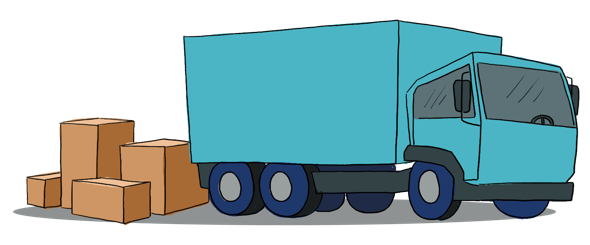
\includegraphics[width=1\linewidth]{Pi5_bai2}
			\vspace*{-15pt}
		\end{figure}
	$\pmb{3.}$ Sau khi được sạc đầy pin, điện thoại di động của bạn An dùng đúng $6$ tiếng ở chế độ trò chuyện hoặc đúng $210$ tiếng ở chế độ chờ. Khi bạn An lên tàu hoả để đi du lịch, pin của bạn được sạc đầy $100\%$, và trên tàu không có ổ cắm sạc nên khi xuống ga, pin của bạn cũng vừa hết sạch. Biết rằng An đã nói chuyện với bạn bè đúng một nửa thời gian khi ngồi trên tàu, còn nửa thời gian còn lại đặt điện thoại ở chế độ chờ. Hỏi thời gian An đi trên tàu hoả là bao nhiêu lâu?
	\begin{figure}[H]
			\centering
			\vspace*{-5pt}
			\captionsetup{labelformat= empty, justification=centering}
			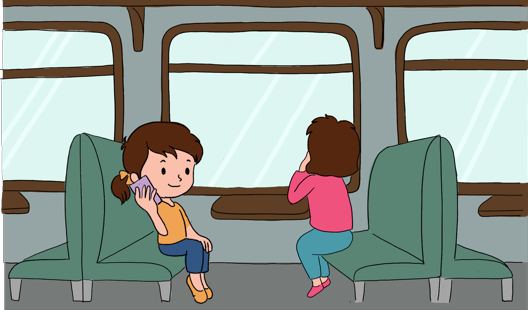
\includegraphics[width=1\linewidth]{Pi5_bai3}
			\vspace*{-15pt}
		\end{figure}
	$\pmb{4.}$ Một nhóm học sinh đi bộ từ điểm hẹn tới bến xe buýt để kịp đón chuyến xe vào lúc $8$ giờ. Cũng vào thời điểm này, từ điểm thăm quan, một chiếc xe buýt cũng xuất phát để tới kịp bến xe đón nhóm học sinh đó. Tuy  nhiên nhóm học sinh tới bến xe buýt khá sớm, vào lúc $6$ giờ $10$ phút, nên họ quyết định đi bộ tiếp tới điểm thăm quan. Trên đường, các bạn đã gặp được xe buýt và lên xe đi tiếp.  Cuối cùng cả nhóm đến được điểm thăm quan sớm hơn $20$ phút so với thời gian ấn định. Biết rằng vận tốc của xe buýt là $60$ km/h và vận tốc đi bộ của các em học sinh luôn không đổi. Hãy tìm vận tốc đi bộ của nhóm học sinh trước khi gặp xe buýt.
	\begin{figure}[H]
			\centering
%			\vspace*{-5pt}
			\captionsetup{labelformat= empty, justification=centering}
			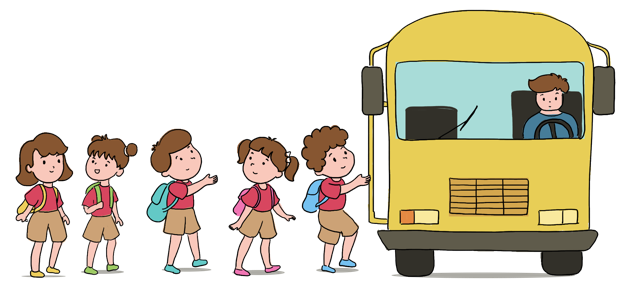
\includegraphics[width=1\linewidth]{Pi5_bai4}
			\vspace*{-10pt}
		\end{figure}
	$\pmb{5.}$ 	Có $100$ chiếc xe ô tô đỗ liền nhau thành một hàng dọc bên lề đường, trong đó có $70$ chiếc xe hiệu Mercedes, còn lại là những xe nhãn hiệu khác. Trong các xe nhãn hiệu Mercedes có $30$ chiếc màu đỏ, $20$ chiếc màu vàng và $20$ chiếc màu hồng. Biết rằng không có hai xe Mercedes nào khác màu lại đỗ cạnh nhau. Em hãy chỉ ra rằng luôn tìm ra $3$ chiếc xe Mercedes cùng màu đỗ liên tiếp nhau.
	\begin{figure}[H]
			\centering
			\vspace*{-5pt}
			\captionsetup{labelformat= empty, justification=centering}
			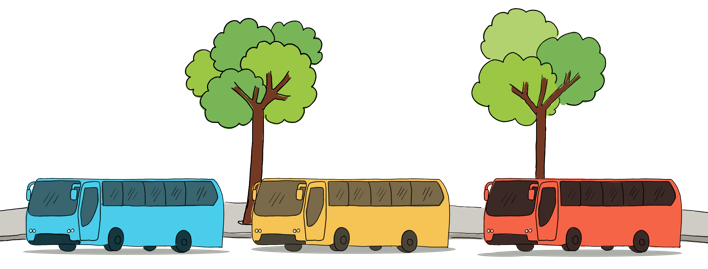
\includegraphics[width=1\linewidth]{Pi5_bai5}
			\vspace*{-15pt}
		\end{figure}
	$\pmb{6.}$ Một lớp học có $20$ em học sinh. Cô giáo chủ nhiệm của lớp tổ chức một số buổi thăm quan vào mỗi ngày cuối tuần trong suốt năm học, mỗi buổi tham quan có ít nhất $4$ em học sinh tham gia. Em hãy chứng minh rằng có một buổi thăm quan mà mỗi em học sinh tham gia buổi đó đều tham gia ít nhất $1/17$ tổng số tất cả các buổi tham quan của cả năm học.
	\begin{figure}[H]
		\centering
		\vspace*{-5pt}
		\captionsetup{labelformat= empty, justification=centering}
		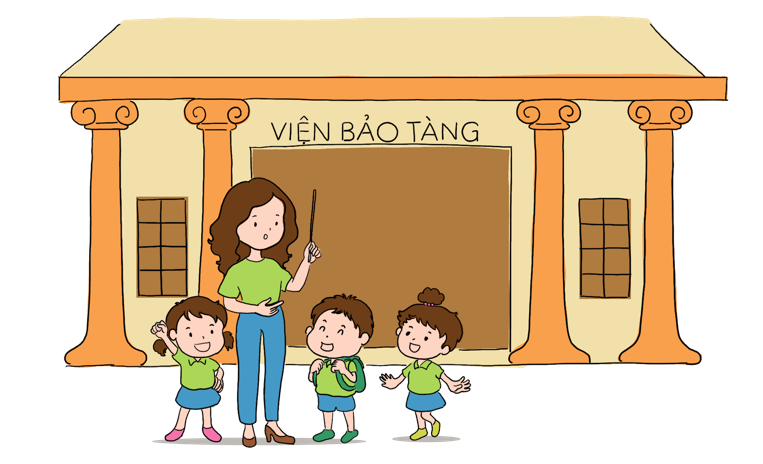
\includegraphics[width=1\linewidth]{Pi5_bai6}
		\vspace*{-15pt}
	\end{figure}
\end{multicols}
\newpage
\begingroup
\AddToShipoutPicture*{\put(110,645){
\includegraphics[scale=1]{../tieude2.pdf}}} 
\centering
\endgroup
\vspace*{55pt}

\begin{multicols}{2}
	$\pmb{1.}$ Một bác nông dân chở một xe ô tô quất cảnh ra chợ Tết để bán. Sau khi bán hết cây quất cuối cùng với giá $230$ nghìn đồng, bác tính nhẩm lại thấy mình đã bán số cây quất với giá trung bì nh là $245$ nghìn đồng/cây. Nhưng ngay lúc ấy người mua cây quất cuối quay trở lại và chỉ cho bác thấy cành quất bị rụng quá nhiều lá, nên ông ta chỉ đồng ý mua với giá $158$ nghìn đồng. 
	Bác chấp thuận và bán cây quất đó. Khi nhẩm tính lại, bác nông dân thấy giá trung bình của xe quất bây giờ là $242$ nghìn đồng. Hỏi bác đã bán được bao nhiêu cây quất?
	\begin{figure}[H]
		\centering
		\vspace*{-10pt}
		\captionsetup{labelformat= empty, justification=centering}
		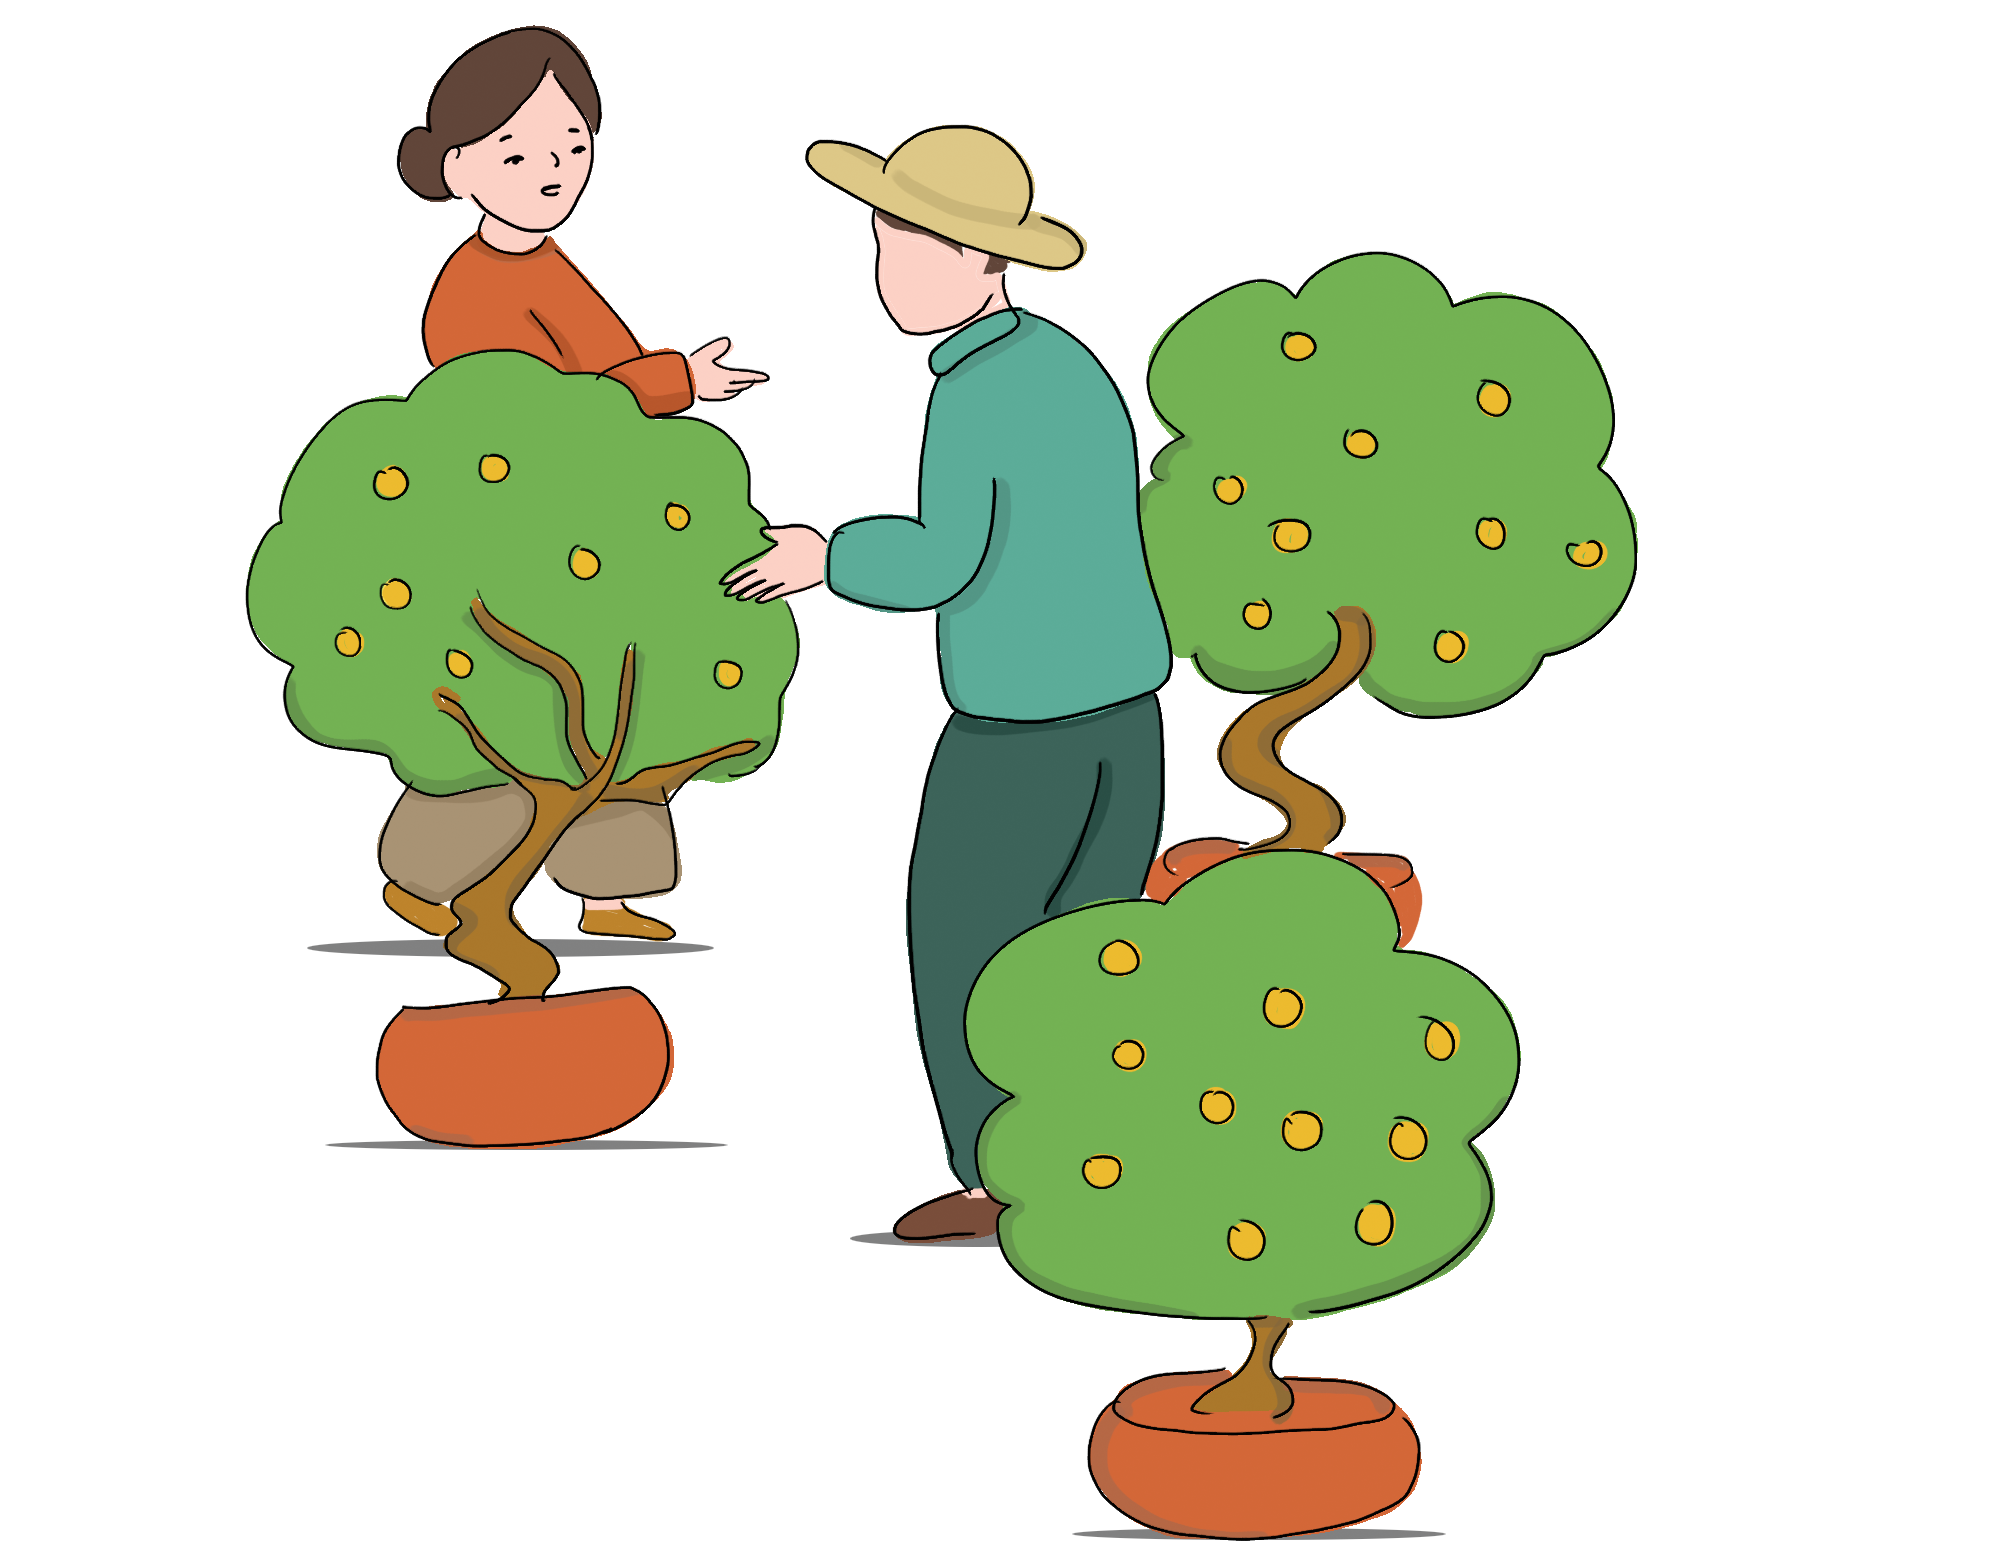
\includegraphics[width=0.7\linewidth]{Pi1_2_Bai1}
		\vspace*{-15pt}
	\end{figure}
	\textit{Lời giải.} Gọi số cây quất là $n$, còn giá tiền một cây quất là $Q$ (nghìn đồng). Khi đó $Q+230 = 245n$ và $Q+ 158 = 242n$. Trừ hai đẳng thức này ta có $72 = 3n$. Suy ra bác nông dân đã bán được $24$ cây quất.
	\vskip 0.1cm
	$\pmb{2.}$ Chuyện kể rằng có một người khi gặp nhà triết học và toán học Hy--Lạp Pythagoras đã hỏi ông: ``Bây giờ là mấy giờ?" Pythagoras đã trả lời ``Cho đến hết ngày, còn lại hai lần của hai phần năm khoảng thời gian đã trôi qua từ lúc bắt đầu ngày". Nghe vậy, người đó chịu không thể nghĩ ra ngay được lúc họ gặp nhau là mấy giờ. Em có thể giúp trả lời lúc đó là mấy giờ được không?
	\vskip 0.1cm
	\textit{Lời giải.} 	Gọi $x$ là thời gian (tính theo giờ) đã trôi qua từ lúc bắt đầu ngày. Khi đó ta có hệ thức sau theo câu trả lời của Pythagoras: $24 - x = 4/5 x$. Suy ra $x = 40/3$ (giờ), có nghĩa là $13$ giờ $20$ phút. Vậy người đó đã gặp Pythagoras lúc $13$ giờ $20$ phút.
	\begin{figure}[H]
		\centering
		\vspace*{-10pt}
		\captionsetup{labelformat= empty, justification=centering}
		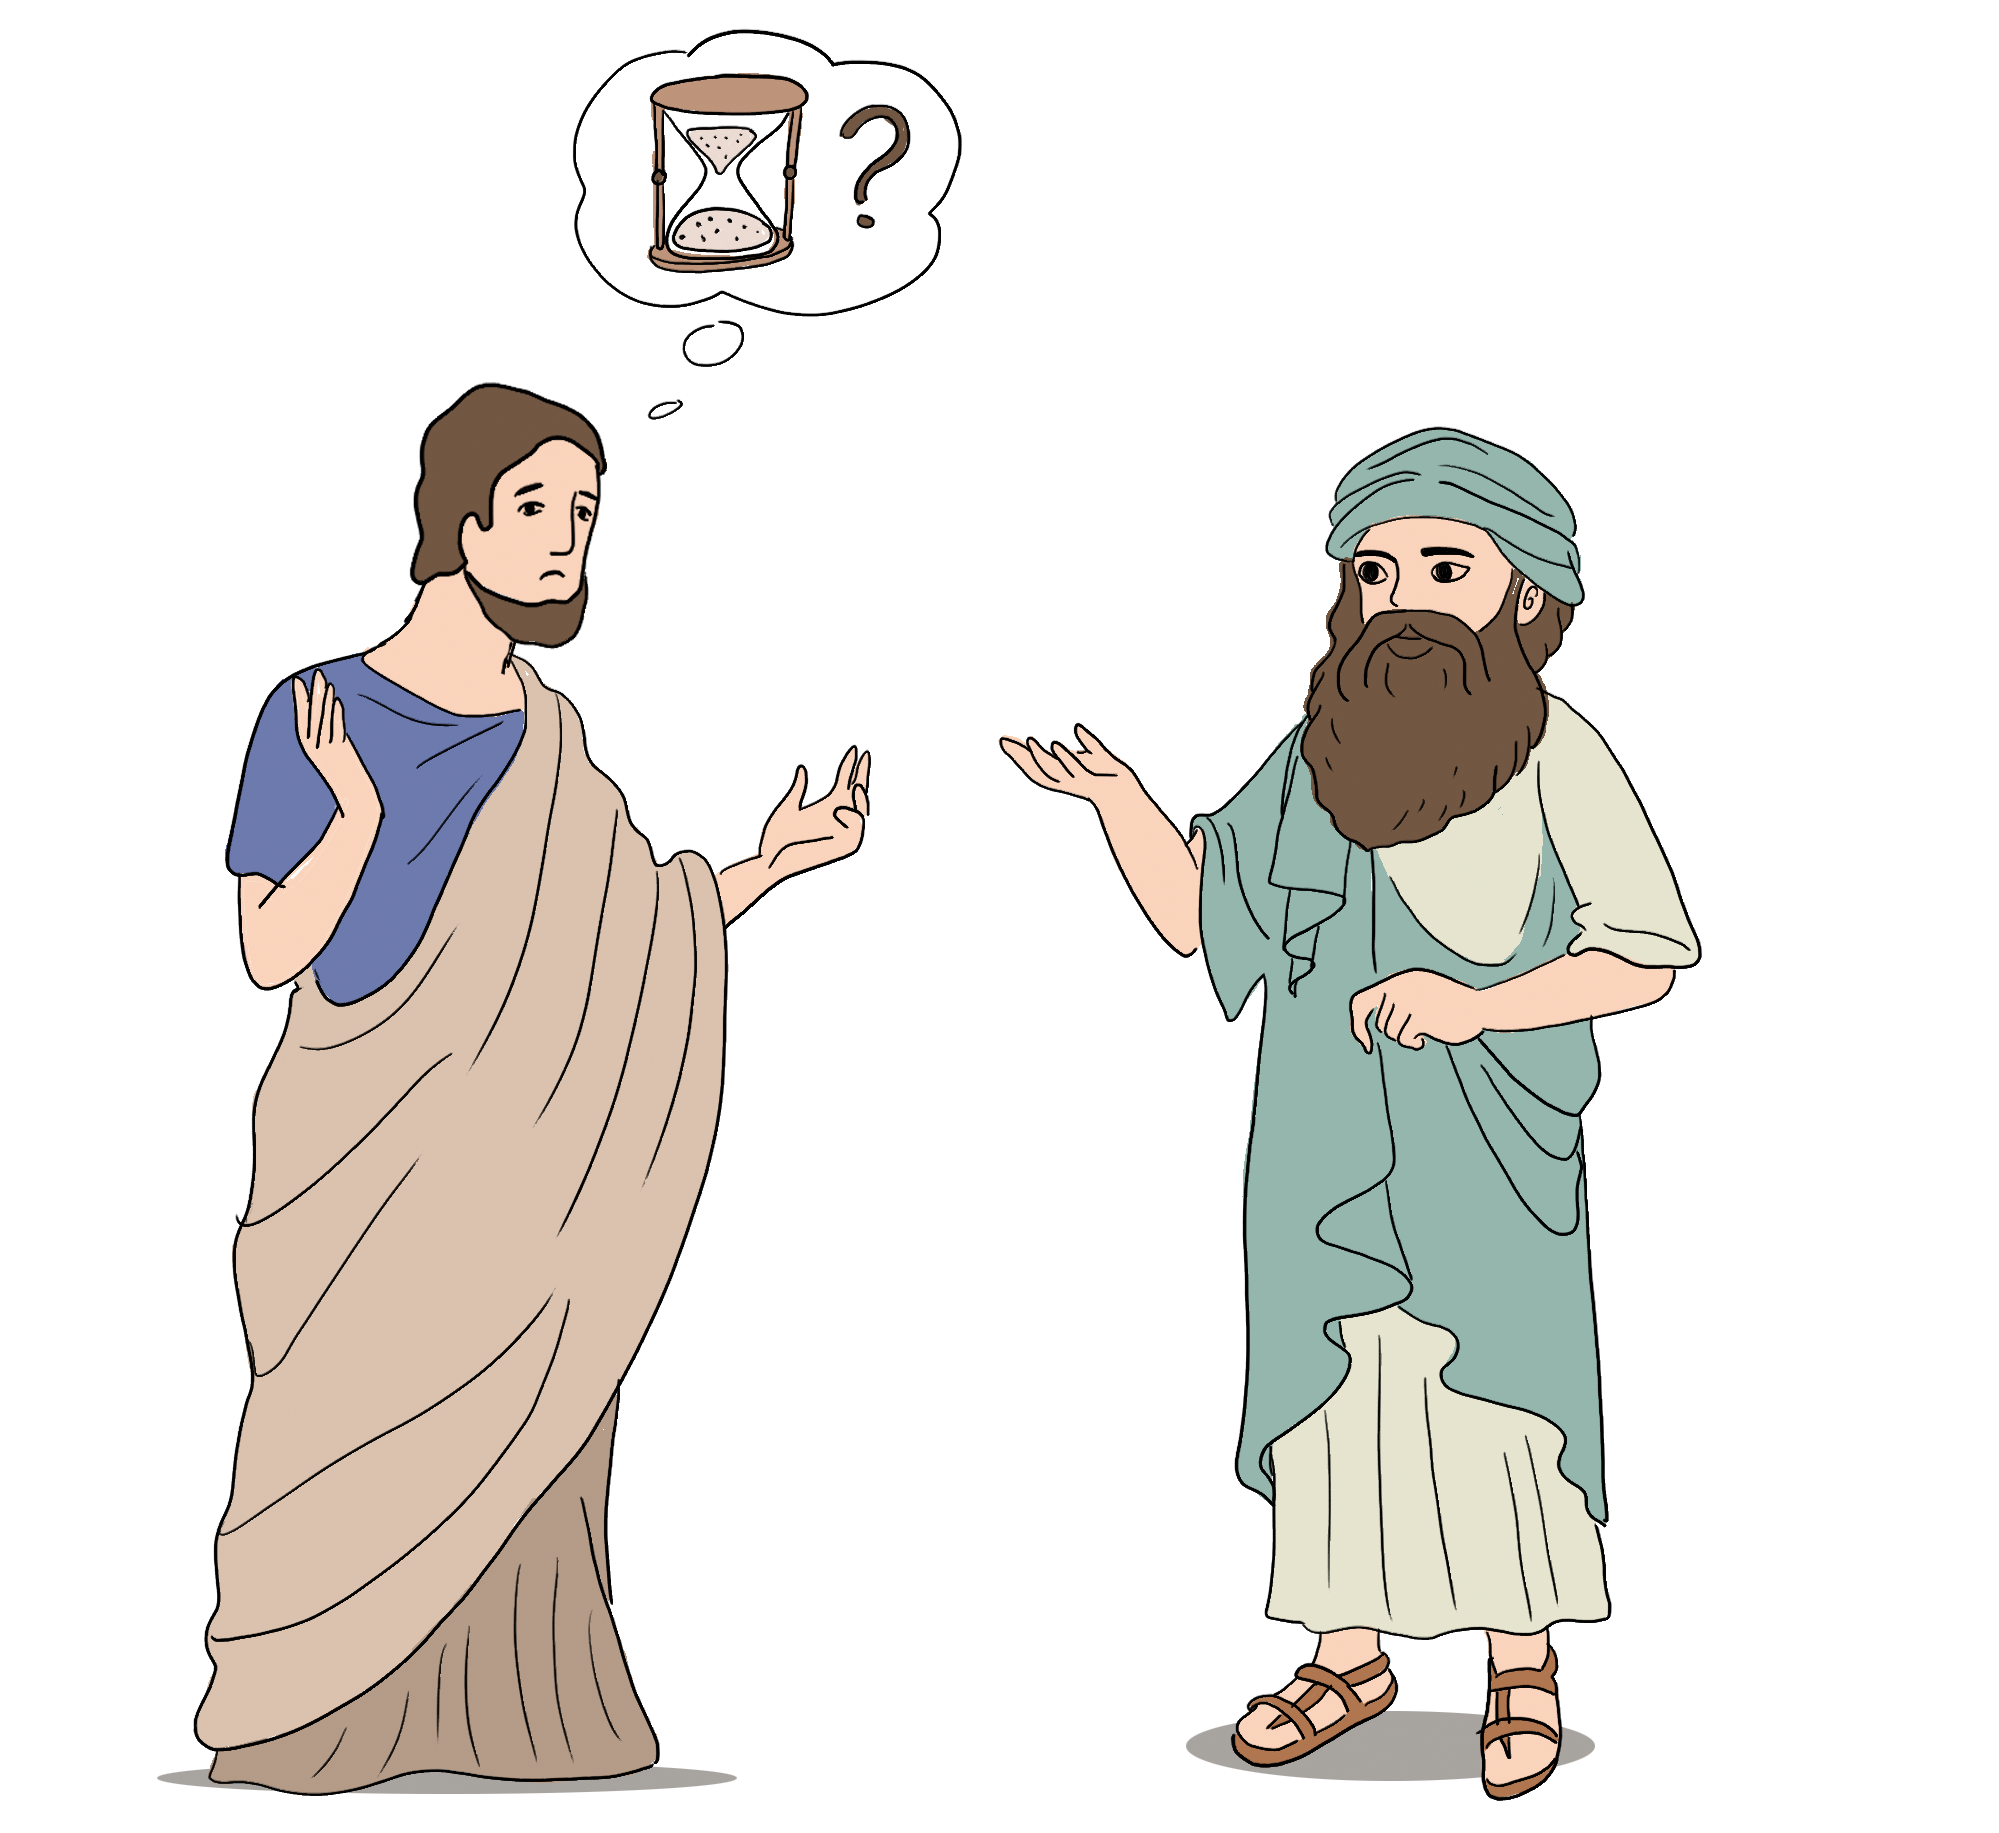
\includegraphics[width=0.6\linewidth]{Pi1_2_Bai2}
		\vspace*{-10pt}
	\end{figure}
	$\pmb{3.}$ Một tháng trước bà Hoa ra chợ mua một cân khoai tây, một cân thịt và một chục trứng. Chủ nhật vừa rồi, khoai tây tăng lên gấp $3$, thịt gấp $4$ lần còn trứng đắt gấp $5$ lần, nên bà Hoa phải trả $600$ nghìn cho từng ấy món hàng như lần thứ nhất. Hôm nay thì khoai lại đắt gấp $6$ lần so với tháng trước, thịt đắt gấp $5$ lần còn trứng chỉ đắt gấp $4$ lần nên bà Hoa lại phải trả $660$ nghìn với cùng một lượng hàng. Hỏi bà Hoa đã trả bao nhiêu tiền cho lần mua thứ nhất?
	\begin{figure}[H]
		\centering
		\vspace*{-10pt}
		\captionsetup{labelformat= empty, justification=centering}
		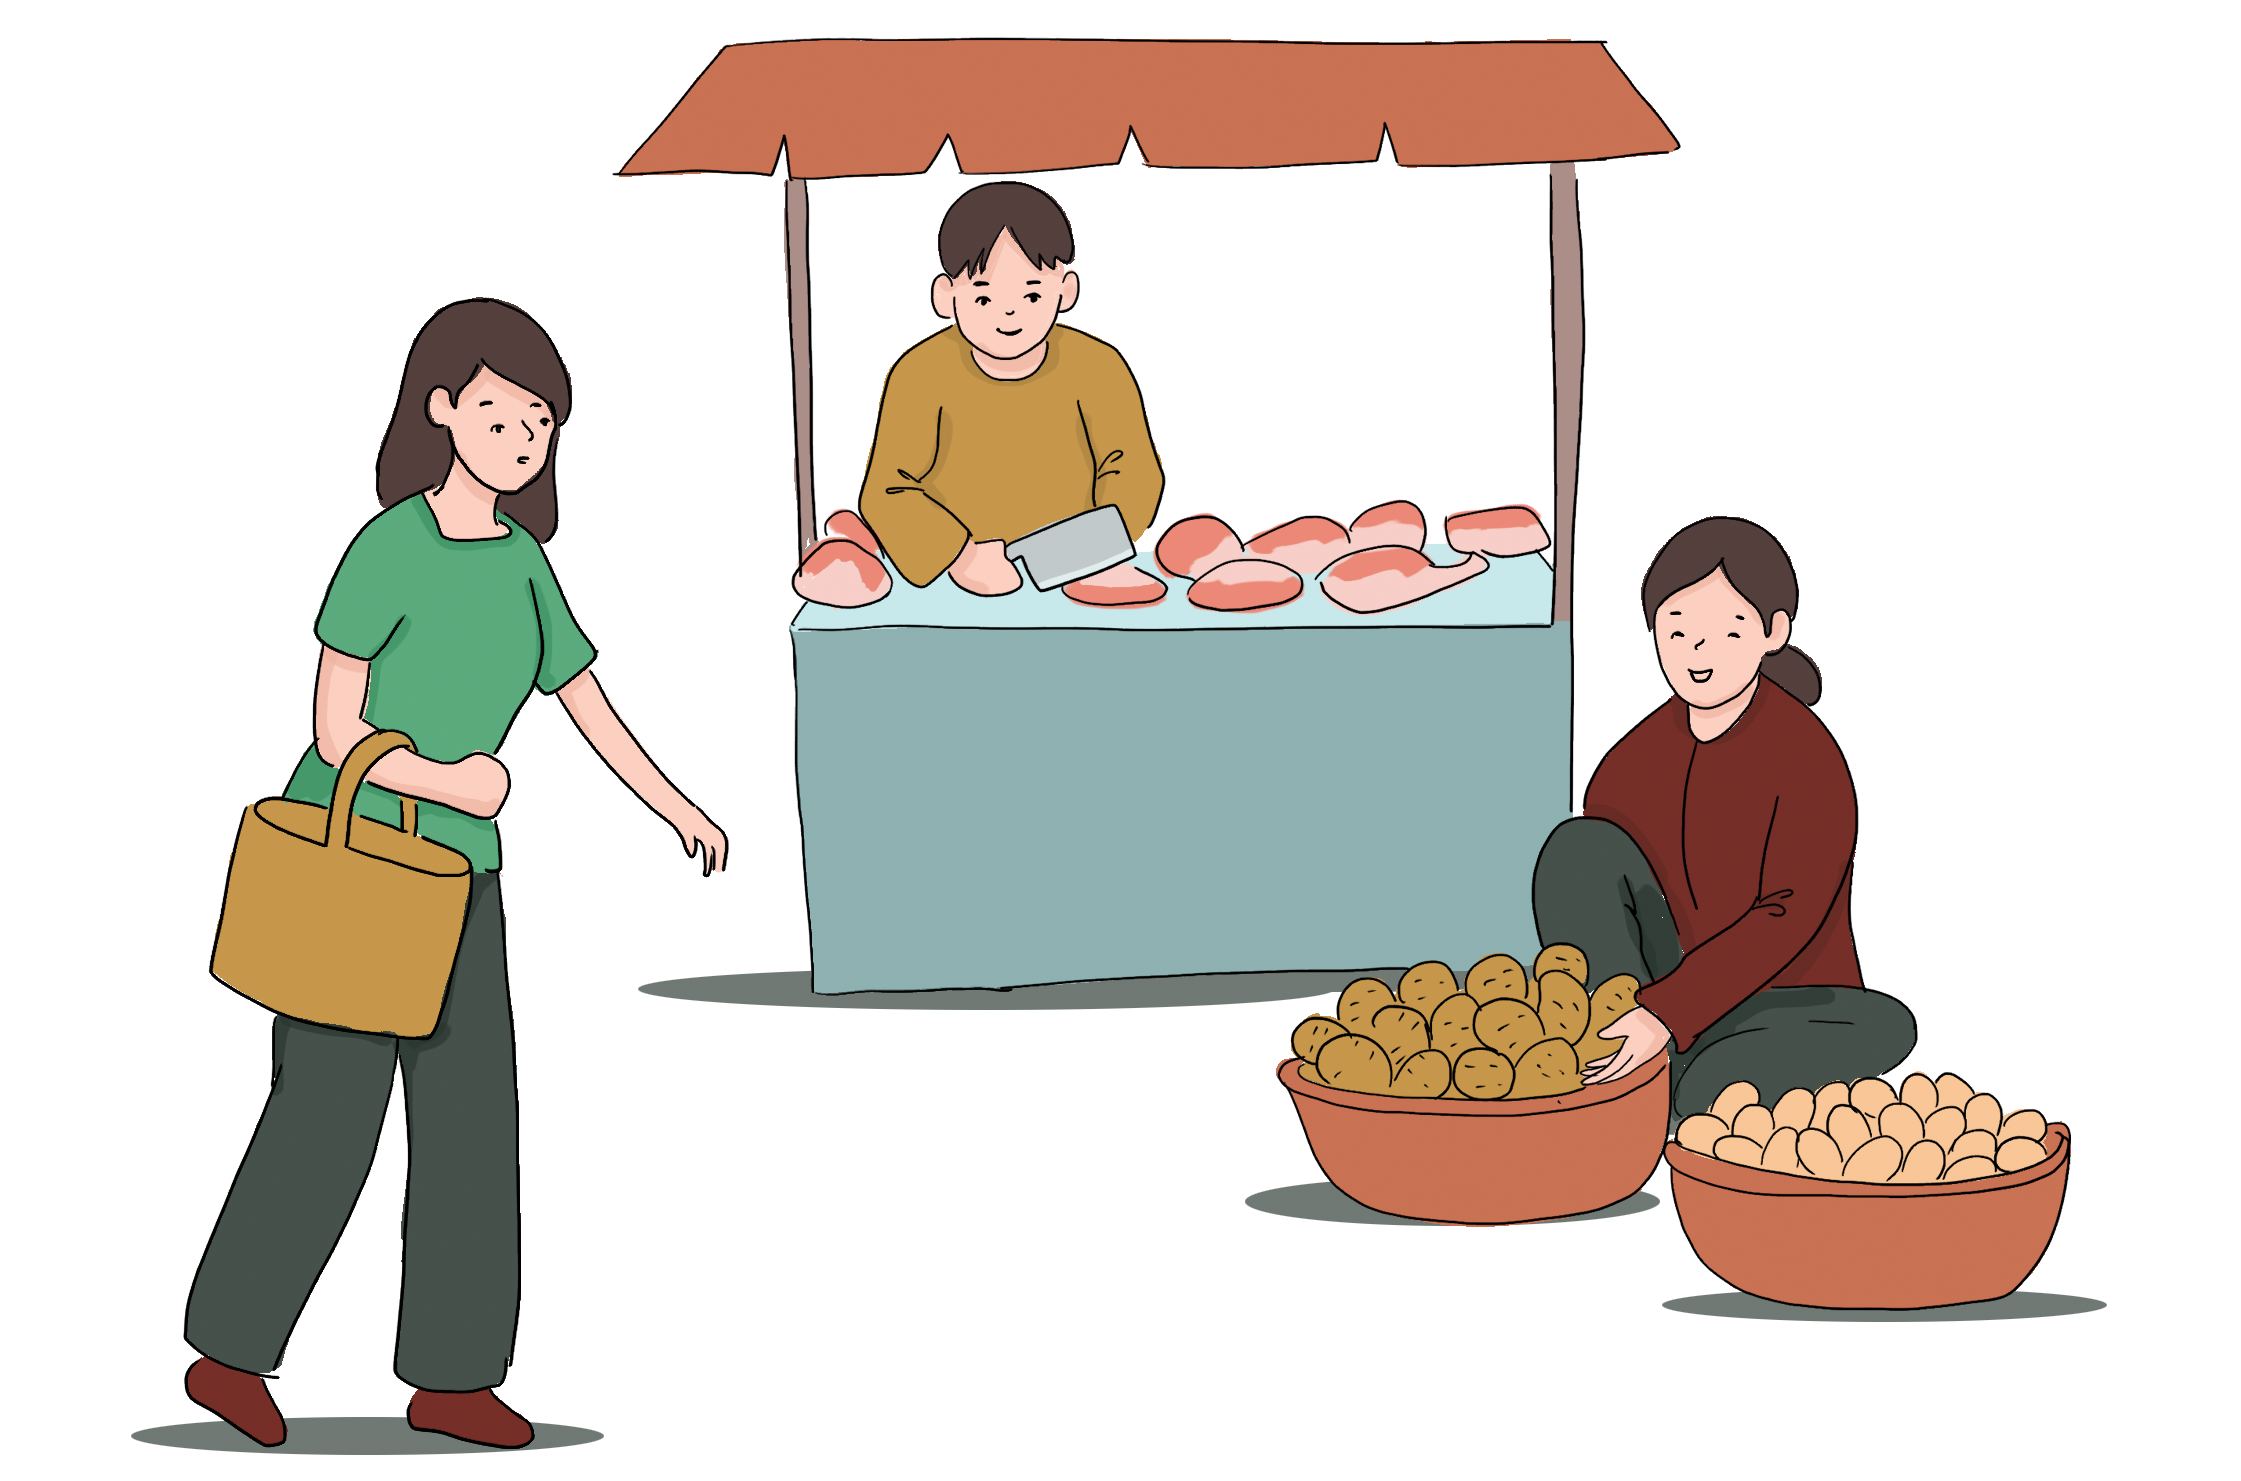
\includegraphics[width=0.7\linewidth]{Pi1_2_Bai3}
		\vspace*{-10pt}
	\end{figure}
	\textit{Lời giải.} 	Giả sử vào tháng trước trong lần mua đầu tiên giá một cân khoai tây là $a$ (nghìn đồng), giá một cân thịt là $b$ (nghìn đồng) và giá một chục trứng là $c$ (nghìn đồng). Khi đó trong lần mua thứ nhất bà Hoa đã trả $a + b + c$ (nghìn), trong lần mua thứ hai là $3a+4b+5c = 600$ và trong lần mua thứ ba là $6a + 5b+ 4c = 660$. Cộng hai đẳng thức cuối này, ta có $9(a+b+c)= 1260$. Suy ra $a+b+c = 140$. Vậy vào tháng trước bà Hoa chỉ phải trả có $140$ nghìn đồng.
	\vskip 0.1cm
	$\pmb{4.}$ Trong một buổi dạ hội nọ mỗi quý ông đã hân hạnh khiêu vũ với ba quý bà, còn mỗi quý bà cũng đã khiêu vũ với ba quý ông. Em hãy chỉ ra rằng số quý ông và số quý bà tham gia dạ hội là bằng nhau.
	\begin{figure}[H]
		\centering
		\vspace*{-5pt}
		\captionsetup{labelformat= empty, justification=centering}
		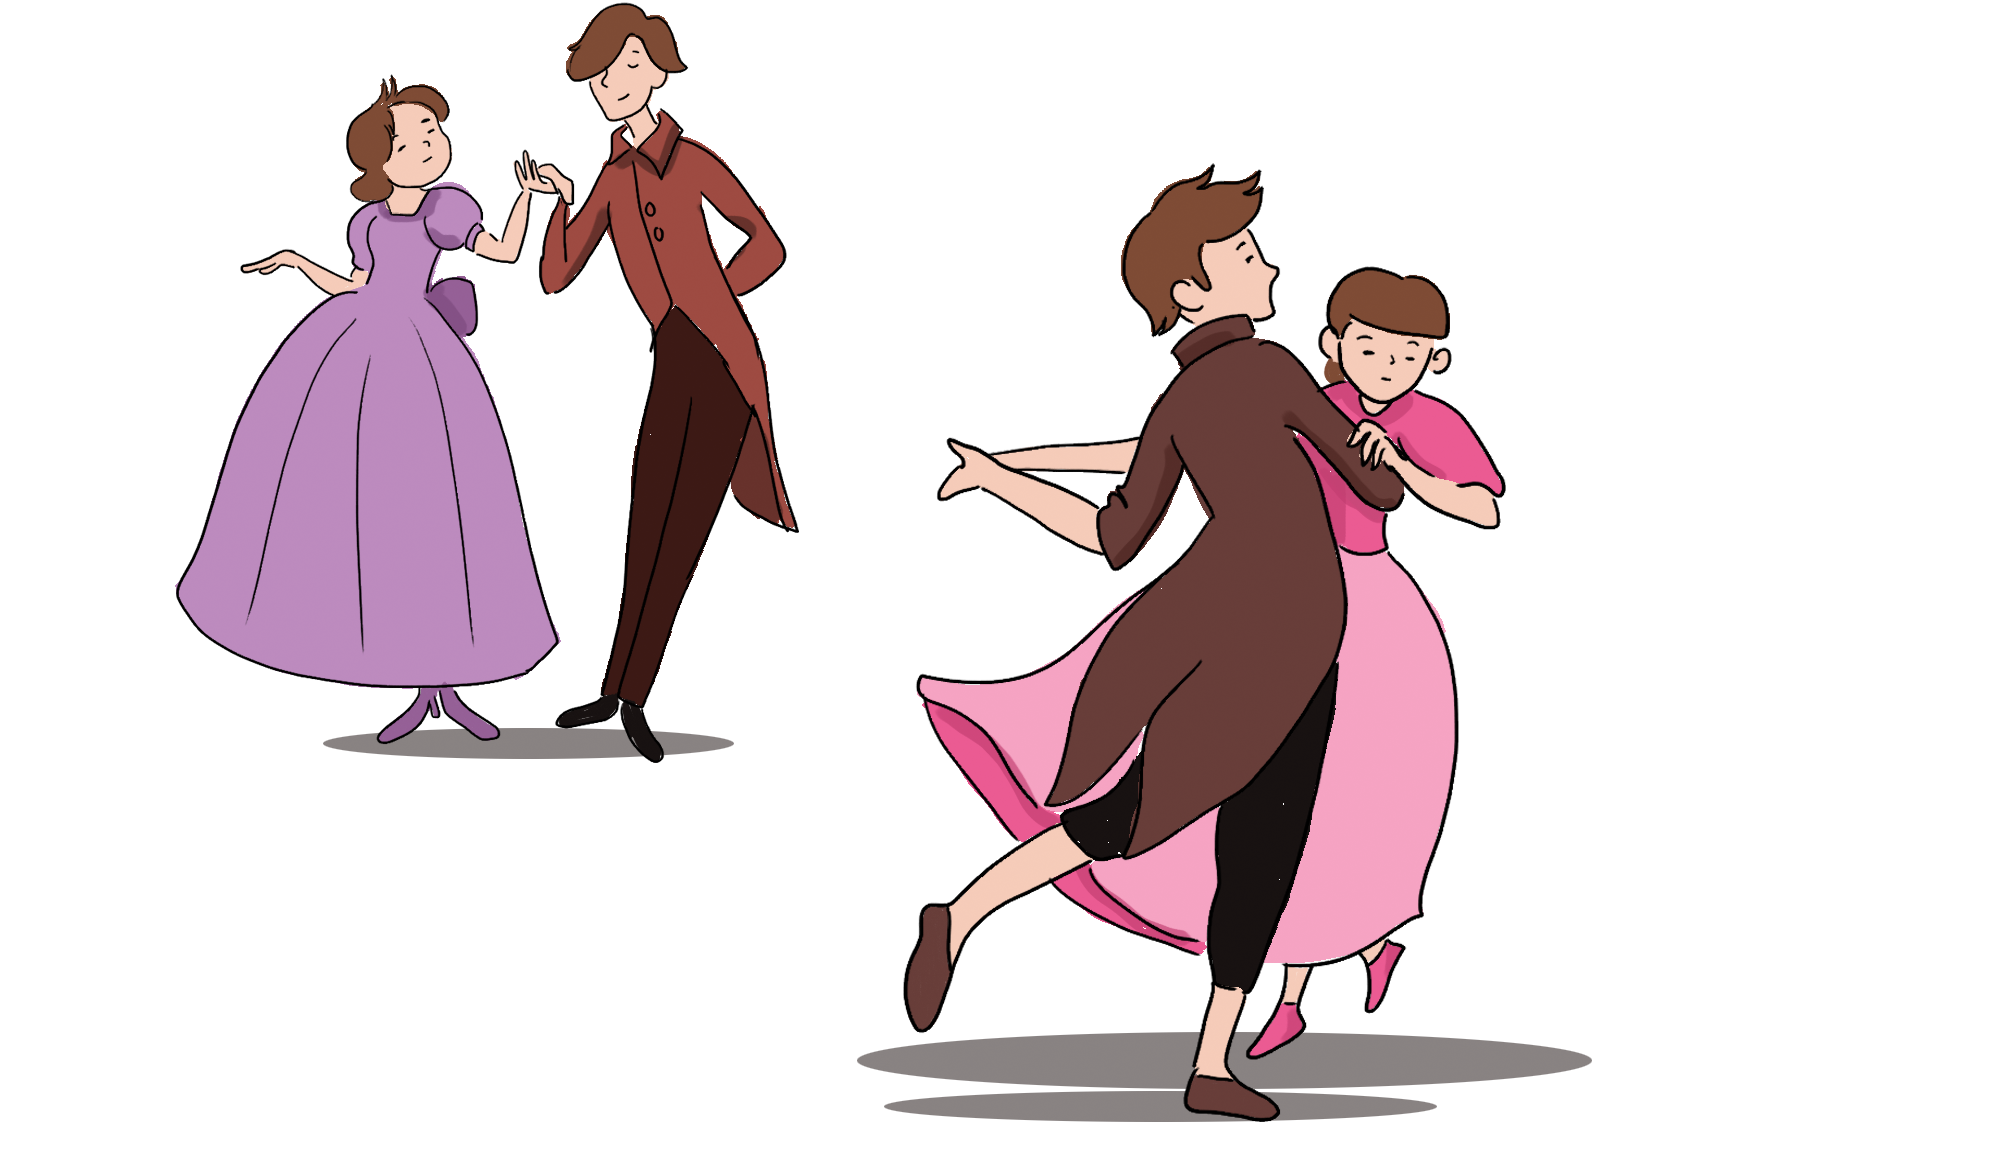
\includegraphics[width=0.85\linewidth]{Pi1_2_Bai4}
		\vspace*{-10pt}
	\end{figure}
	\textit{Lời giải.} Ta sẽ tính tổng tất cả các cặp đã khiêu vũ với nhau. Một mặt, tổng này sẽ bằng $3$ lần số các quý ông, mặt khác nó lại bằng $3$ lần số các quý bà. Vì thế số các quý ông bằng số các quý bà.
	\vskip 0.1cm
	$\pmb{5.}$ 	Sau khi kết thúc một giải thi cờ vua, ban tổ chức nhận thấy mỗi kỳ thủ tham gia đã có số trận thắng khi chơi bằng quân trắng bằng đúng tổng số trận thắng của toàn bộ các kỳ thủ còn lại khi chơi quân đen. Em hãy chỉ ra rằng tất cả các kỳ thủ tham gia thi đấu đã có số trận thắng là như nhau.
	\begin{figure}[H]
		\centering
		\vspace*{-5pt}
		\captionsetup{labelformat= empty, justification=centering}
		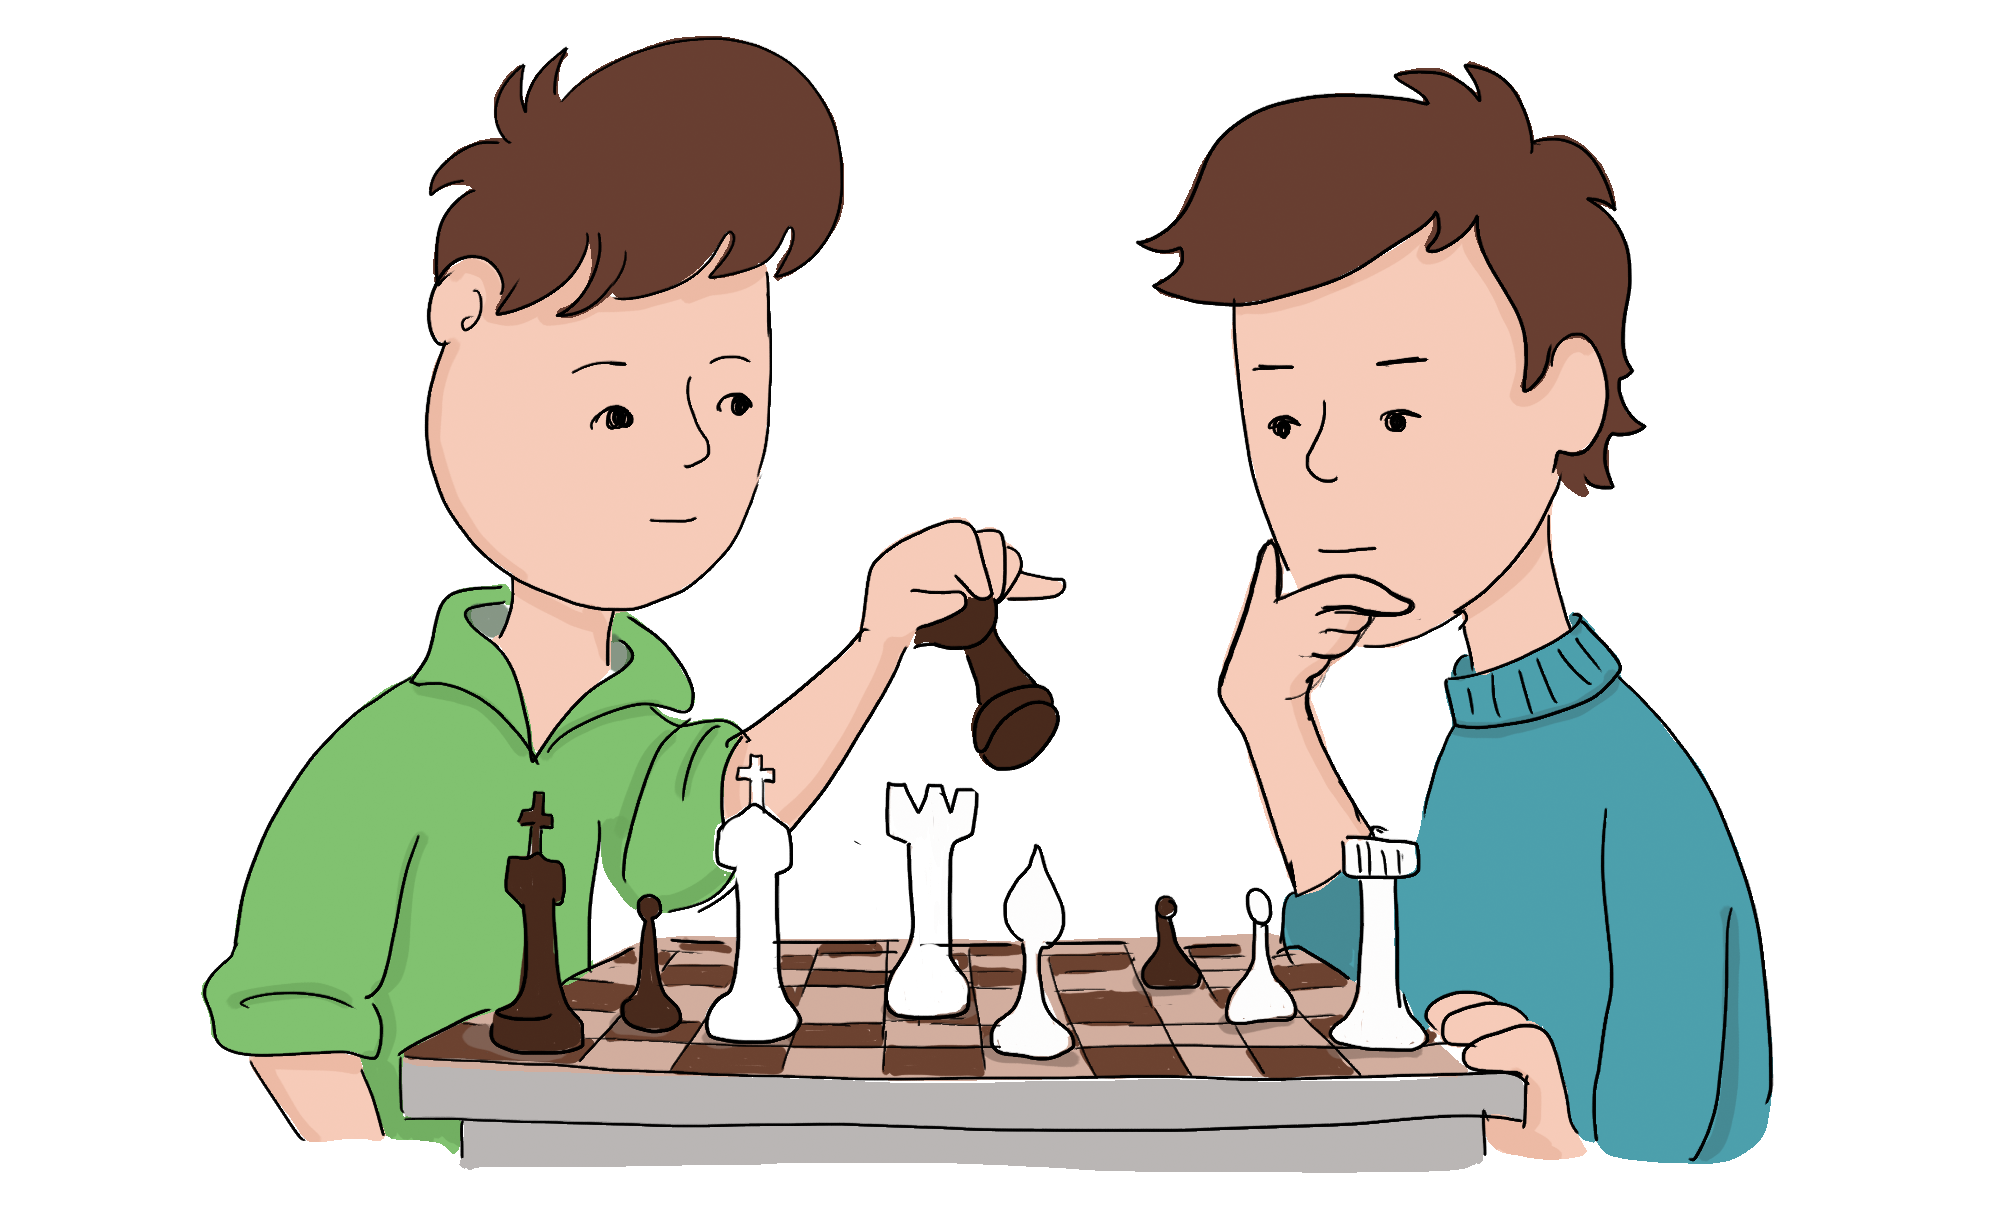
\includegraphics[width=0.6\linewidth]{Pi1_2_Bai5}
		\vspace*{-10pt}
	\end{figure}
	\textit{Lời giải.} Các em có thể nhận thấy số trận thắng của mỗi kỳ thủ tham gia giải bằng đúng tổng số trận thắng của tất cả các kỳ thủ khi chơi bằng quân đen. Vì thế mọi kỳ thủ tham gia đã có số trận thắng bằng nhau.
	\vskip 0.1cm
	$\pmb{6.}$ Vào một ngày Chủ nhật nọ, Vinh và người em trai nhỏ tuổi hơn là Minh  đạp hai chiếc xe tới hiệu sách trung tâm cách nhà vài cây số. Tại đó mỗi người chọn mua một cuốn sách quý mà nhóm bạn bè cũ đang bàn luận khen ngợi thường xuyên mấy năm nay trên Facebook. Mỗi người đều lấy tổng tất cả các chữ số của tất cả các trang sách mình đã mua và nhận thấy rằng số đó bẳng năm sinh của mình. Vậy ai  trong số hai anh em Vinh và Minh  đang đi học lớp  bồi dưỡng Toán cho học sinh phổ thông nhỉ?
	\begin{figure}[H]
		\centering
		\vspace*{-5pt}
		\captionsetup{labelformat= empty, justification=centering}
		
\includegraphics[width=0.8\linewidth]{Pi1_2_Bai6}
		\vspace*{-10pt}
	\end{figure}
	\textit{Lời giải.} 	Trước tiên ta tính tổng chữ số của tất cả các số từ $1$ tới $99$. Nhận thấy rằng mỗi chữ số, trừ chữ số $0$ đều xuất hiện $10$ lần ở hàng chục, và cũng $10$ lần ở hàng đơn vị, nghĩa là $20$ lần tổng cộng. Do $1+2+ \cdots+9=45$, nên tổng này bằng  $900$. Tổng các chữ số của các số từ $100$ tới $199$ sẽ lớn hơn tổng trước là $100$. Vì thế tổng các chữ số của các số từ $1$ tới $199$ bằng $1900$. Vì vậy ta xét một vài trường hợp sau.
	\begin{table}[H]
		\centering
		\vspace*{-5pt}
		\captionsetup{labelformat= empty, justification=centering}
		\renewcommand{\arraystretch}{1.05}
		\begin{tabular}{|l|l|}
			\hline
			\textbf{Số trang sách}&	\textbf{Tổng các chữ số}\\
			\hline
			$200$&	$1900+2 =1902$\\
			\hline
			$202$&	$1902+3+4=1909$\\
			\hline
			$204$&	$1909+5+6=1920$\\
			\hline
			$206$&	$1920+7+8=1935$\\
			\hline
			$208$&	$1935+9+10=1954$\\
			\hline
			$210$&	$1954+11+3=1968$\\
			\hline
			$212$&	$1968+4+5=1977$\\
			\hline
			$214$&	$1977+6+7=1990$\\
			\hline
			$216$&	$1990+8+9=2007$\\
			\hline
			$217$&	$2007+10=2017$\\
			\hline
			$218$&	$2017+11=2028$\\
			\hline
		\end{tabular}
		\vspace*{-5pt}
	\end{table}
	Các em thấy ngay chỉ có người sinh năm $2007$ trong số hai anh em mới có thể là học sinh phổ thông. Người đó cũng không thể là anh, vì nếu vậy người em trai sinh năm $2017$ đến giờ mới có $5$ tuổi không thể tự đi xe đạp vài km để mua sách dày hơn hai trăm trang và về nhà tự làm tính cộng hết từng đó chữ số, hơn nữa lại có nhóm bạn bè cũ trên Facebook bàn luận về cuốn sách tới mấy năm rồi. Vì vậy các em kết luận được người sinh năm $2007$ là em và có tên là Minh.
\end{multicols}
\newpage
\begingroup
\thispagestyle{toancuabinone}
\blfootnote{$^1$\color{toancuabi}Ottawa, Canada.}
\AddToShipoutPicture*{\put(60,733){
\includegraphics[width=17.2cm]{../mathc.pdf}}}
%\AddToShipoutPicture*{\put(-2,733){
\includegraphics[width=17.2cm]{../mathl.pdf}}} 
\AddToShipoutPicture*{\put(140,675){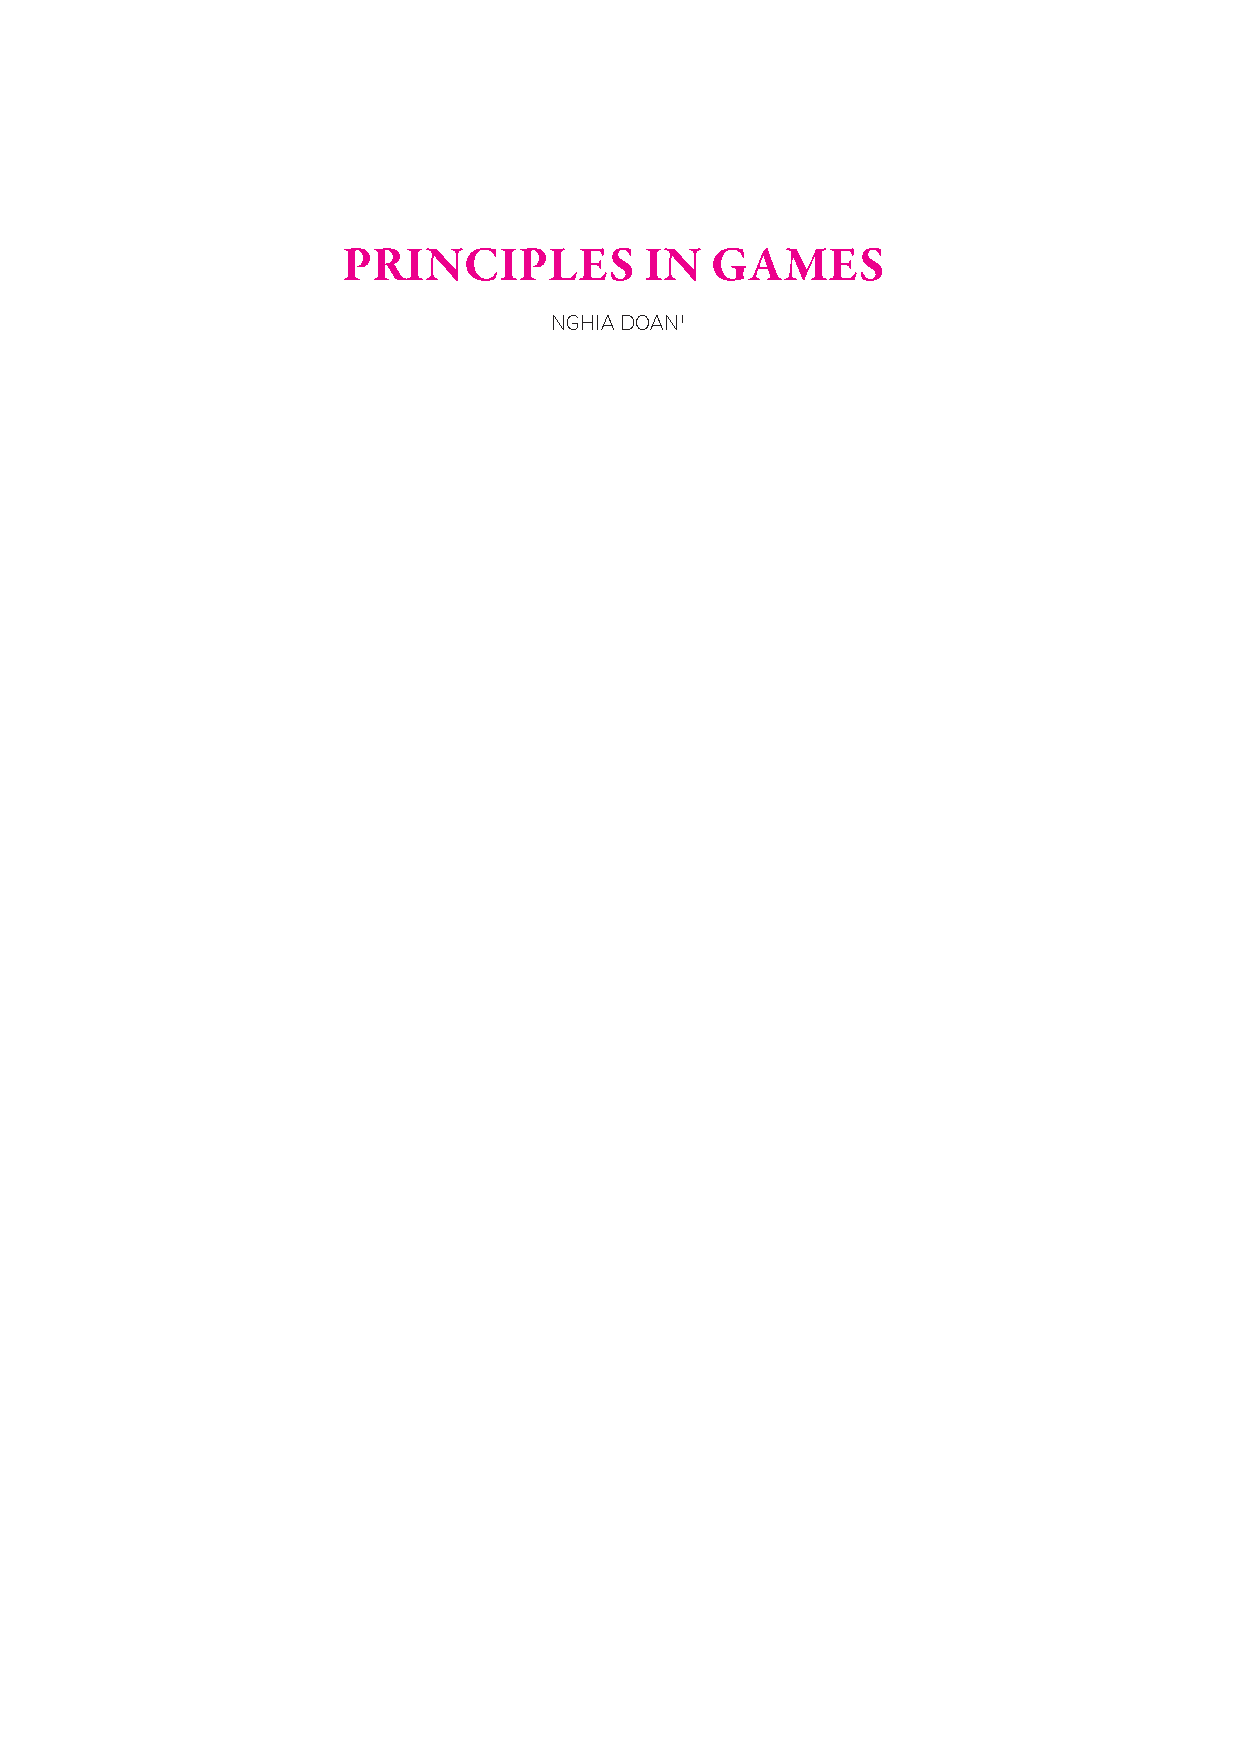
\includegraphics[scale=1]{../tieude6.pdf}}} 
\centering
\endgroup
\graphicspath{{../toancuabi/pic/}}
\vspace*{33pt}

\begin{multicols}{2}
	In this article, we discuss a few games and principles associated with solutions to the problems posed by the games.
	\vskip 0.2cm
	\PIbox{{\color{toancuabi}\textbf{Example} (Pigeons share a hole)\textbf{.}}
		Each square of a $3 \times 3$ board is filled with one of the numbers $-1, 0, +1$. See the figure below for an example.
		Viet calculates the sums of the rows, columns, and two main diagonals. He found that there are at least two equal sums.
		For example, in the example below, both the sums of the second and third rows are $0$.
		Is it always true that there are at least two equal sums?}
	\vskip 0.1cm
	\begin{figure}[H]
		\vspace*{-5pt}
		\centering
		\captionsetup{labelformat= empty, justification=centering}
		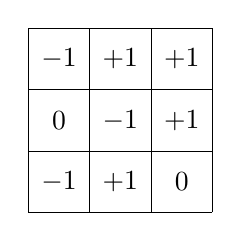
\begin{tikzpicture}[scale=0.78]
			\draw (0,0) grid (3,3);
			\draw (0.5,0.5) node {$-1$};
			\draw (1.5,0.5) node {$+1$};
			\draw (2.5,0.5) node {$0$};
			\draw (0.5,1.5) node {$0$};
			\draw (1.5,1.5) node {$-1$};
			\draw (2.5,1.5) node {$+1$};
			\draw (0.5,2.5) node {$-1$};
			\draw (1.5,2.5) node {$+1$};
			\draw (2.5,2.5) node {$+1$};
		\end{tikzpicture}
		\vspace*{-10pt}
	\end{figure}
	\textit{Solution.}
	The answer is yes. The largest possible sum is $3$ and the smallest is $-3.$
	So there are0 $7$ possible values $-3,-2,\ldots,2,3$ for $8$ sums, so two of them should be the same and therefore equal.
	\vskip 0.1cm	
	In above we applied the \textit{Pigeonhole principle: if $n+1$ or more pigeons are placed in $n$ holes, then one hole must contain two or more pigeons.} 
	\vskip 0.2cm
	\PIbox{{\color{toancuabi}\textbf{Example} (Nothing ever changes)\textbf{.}}
	Each square of the  board contains a $+$ or $-$ signs, see the board the left,
	which contains a single $-$ at the square intersection of the first row and second column.}
	\vskip 0.1cm
	\vspace*{0.1pt}
	\vspace*{-8pt}
	\PIbox{
	At each step, you can change all the signs in a row, a column, or a diagonal to their opposite ones, i.e. $+$ to $-$, and $-$  to $+$.
	An example of how a column is changed shown as below in the board on the right.}
	\begin{center}
		\begin{tikzpicture}[scale=0.78]
			\draw [fill=cackithi!50] (1,0) rectangle (2,4);
			\draw [fill=cackithi!50] (6,0) rectangle (7,4);
			\draw (0,0) grid (4,4);
			\draw (0.5,0.5) node {$+$};
			\draw (1.5,0.5) node {$+$};
			\draw (2.5,0.5) node {$+$};
			\draw (3.5,0.5) node {$+$};
			\draw (0.5,1.5) node {$+$};
			\draw (1.5,1.5) node {$+$};
			\draw (2.5,1.5) node {$+$};
			\draw (3.5,1.5) node {$+$};
			\draw (0.5,2.5) node {$+$};
			\draw (1.5,2.5) node {$+$};
			\draw (2.5,2.5) node {$+$};
			\draw (3.5,2.5) node {$+$};
			\draw (0.5,3.5) node {$+$};
			\draw (1.5,3.5) node {$-$};
			\draw (2.5,3.5) node {$+$};
			\draw (3.5,3.5) node {$+$};
			\draw (5,0) grid (9,4);
			\draw (5.5,0.5) node {$+$};
			\draw (6.5,0.5) node {$-$};
			\draw (7.5,0.5) node {$+$};
			\draw (8.5,0.5) node {$+$};
			\draw (5.5,1.5) node {$+$};
			\draw (6.5,1.5) node {$-$};
			\draw (7.5,1.5) node {$+$};
			\draw (8.5,1.5) node {$+$};
			\draw (5.5,2.5) node {$+$};
			\draw (6.5,2.5) node {$-$};
			\draw (7.5,2.5) node {$+$};
			\draw (8.5,2.5) node {$+$};
			\draw (5.5,3.5) node {$+$};
			\draw (6.5,3.5) node {$+$};
			\draw (7.5,3.5) node {$+$};
			\draw (8.5,3.5) node {$+$};
		\end{tikzpicture}
	\end{center}
	\textit{Solution.}
	Take a look at the squares colored \textcolor{red!50}{red}.
	\begin{center}
		\begin{tikzpicture}[scale=0.78]
			\draw [fill=cackithi!50] (1,0) rectangle (2,4);
			\draw [fill=cackithi!50] (6,0) rectangle (7,4);
			\draw [fill=red!50] (0,1) rectangle (1,3);
			\draw [fill=red!50] (1,3) rectangle (3,4);
			\draw [fill=red!50] (3,3) rectangle (4,1);
			\draw [fill=red!50] (3,1) rectangle (1,0);
			\draw (0,0) grid (4,4);
			\draw (0.5,0.5) node {$+1$};
			\draw (1.5,0.5) node {$+1$};
			\draw (2.5,0.5) node {$+1$};
			\draw (3.5,0.5) node {$+1$};
			\draw (0.5,1.5) node {$+1$};
			\draw (1.5,1.5) node {$+1$};
			\draw (2.5,1.5) node {$+1$};
			\draw (3.5,1.5) node {$+1$};
			\draw (0.5,2.5) node {$+1$};
			\draw (1.5,2.5) node {$+1$};
			\draw (2.5,2.5) node {$+1$};
			\draw (3.5,2.5) node {$+1$};
			\draw (0.5,3.5) node {$+1$};
			\draw (1.5,3.5) node {$-1$};
			\draw (2.5,3.5) node {$+1$};
			\draw (3.5,3.5) node {$+1$};
			\draw (5,0) grid (9,4);
			\draw (5.5,0.5) node {$+1$};
			\draw (6.5,0.5) node {$-1$};
			\draw (7.5,0.5) node {$+1$};
			\draw (8.5,0.5) node {$+1$};
			\draw (5.5,1.5) node {$+1$};
			\draw (6.5,1.5) node {$-1$};
			\draw (7.5,1.5) node {$+1$};
			\draw (8.5,1.5) node {$+1$};
			\draw (5.5,2.5) node {$+1$};
			\draw (6.5,2.5) node {$-1$};
			\draw (7.5,2.5) node {$+1$};
			\draw (8.5,2.5) node {$+1$};
			\draw (5.5,3.5) node {$+1$};
			\draw (6.5,3.5) node {$+1$};
			\draw (7.5,3.5) node {$+$};
			\draw (8.5,3.5) node {$+1$};
		\end{tikzpicture}
	\end{center}	
	If we replace the $+$ sign by $+1$ and the $-$ sign by $-1$, then at the beginning the product of all numbers in these red square is $-1.$ 
	Easy to see that each operation to change all the signs in a row, a column or a diagonal shall change exactly two red squares.
	Whatever the numbers in the two red squares, the product of their negates remain same.
	Since the product of the red squares at the beginning is $-1,$ so it cannot be changed at all.
	\vskip 0.1cm
	In above we applied the \textit{Invariant Principle: In mathematics, an invariant is a property of a mathematical object
	(or a class of mathematical objects) which remains unchanged after operations or transformations of a certain type are applied to the objects.} 
	\vskip 0.2cm
	\PIbox{{\color{toancuabi}\textbf{Example} (Integers are well--ordered)\textbf{.}}
	On a stormy night, ten students from the \textit{Math, Chess, and Coding Club in Ottawa} went to a party.
	They left their shoes in the foyer in order to keep the carpet clean. After the dinner, there was a power outage.
	So the students, leaving one by one, put on, at random, any pair of shoes big enough for their feet (each pair of shoes stay together).
	Any student who couldn't find a pair of shoes big enough spent the night at the place of the party.
	\vskip 0.1cm	
	What is the largest number of students who might have had to spend the night? Show an example for this number.
	\textit{Note that no two students wear the same size shoes.}}
	\vskip 0.2cm
	\textit{Solution.}
	Easy to see that if the five students with smallest feet left first wearing all five largest pairs of shoes
	then none of the remaining student can find a pair of shoes to leave.
	Now let assume that there were $6$ students who would have to spent the night and there were $6$ pairs of shoes left,
	then because $6 + 6 > 10,$ so there is a student with his pair of shoes is still at the place of the party. This is not possible!
	\vskip 0.1cm
	In above we applied the \textit{Well--Ordering Principle: the positive integers are well--ordered.
	An ordered set is said to be well--ordered if each and every nonempty subset has a smallest or least element.} 
	\vskip 0.2cm
	\PIbox{{\color{toancuabi}\textbf{Example} (Invariant to reach end--state with desired outcomes)\textbf{.}}
	In a darkroom there are two tables. The first one is empty and the second one is cover by a layer of nickels
	(one nickel thick, so no coin is on top of another), in which $31$ coins are tails up and the rest are heads up.}
	\vskip 0.1cm
	\PIbox{
	Minh enters the room with the task of transferring some coins from the second table to the first table
	(he wears gloves, so he cannot feel the faces of the coins). He can flip over any number of coins when transferring them.
	\vskip 0.1cm
	Is that possible when he leaves the room the number of nickels that are tails up is the same on both tables?}
	\vskip 0.2cm
	\textit{Solution.}
	If Minh turns a coin on the second table during transfer to the first one,
	then the number of coins \textit{tails--up} on the second table will be reduce by one if it was a \textit{tails--p} coin,
	or the number of coins \textit{tails--up} on the first table is increased by one if it was a \textit{heads--up} coin.
	In any case, the difference between the \textit{tails--up} coins on the second and first tables will be reduced by one
	(this is an \textit{invariant}.) Hence, after $31$ moves, they will be the same.
	\vskip 0.1cm
	In above we again applied the \textit{Invariant Principle} with a twist.
	Note that in every turn the difference between the \textit{tails--up} coins on the second and first tables will be reduced by one,
	since at the beginning, in other words, at the \textit{start state} this difference is $31,$
	thus after $31$ turns the game reaches the \textit{end--state} where the difference is $0.$
	\vskip 0.2cm
	\PIbox{{\color{toancuabi}\textbf{Example} (Winning positions)\textbf{.}}
	Berry and Cherry take alternate turns in playing a two--player game removing marbles from a pile as follows:
	\vskip 0.1cm
	$\bullet$ Berry always goes first.
	\vskip 0.1cm
	$\bullet$ The player whose turn it is, must remove exactly $2$, $4$, or $5$ marbles from the pile.
	\vskip 0.1cm
	$\bullet$ The player who at some point is unable to make a move (cannot remove $2$, $4$, or $5$ marbles from the pile) loses the game.
	\vskip 0.1cm
	They play $14$ games with $\{8, 9, \ldots, 21\}$ as the initial number of marbles in the pile.
	What games does Cherry win, regardless of what Berry does?}
	\vskip 0.2cm
	\textit{Solution.}
	The positive integers from $0$ to $21$ can be divided into 7 groups of numbers based on their remainders when divided by $7$,
	\begin{align*}
		&G_0=\{0,7,14,21\}, &&G_1=\{1,8,15\},\\
		& G_2=\{2,9,16\}, &&G_3=\{3,10,17\},\\
		& G_4=\{4,11,18\},&&G_5=\{5,12,19\},\\
		& G_6=\{6,13,20\}
	\end{align*}
	It is easy to verify that,
	\vskip 0.2cm
	\PIbox{\textbf{\color{toancuabi}Claim.}
		If $n$ is a number in $G_0$ and $G_1$ then $n-2$, $n-4$, and $n-5$ are in $G_2,G_3,G_4,G_5,$ or $G_6$.}
	\vskip 0.2cm
	Now, by the rules of the game, it is obvious that $\{0, 1\}$ are \textit{losing} positions and $\{2,4,5\}$ are \textit{winning} positions.
	Furthermore, because $3-2=6-5=1$, so $\{3,6\}$ are also \textit{winning} positions, too.
	\vskip 0.1cm
	Therefore $G_0$ and $G_1$ contain all \textit{losing} positions, while $G_2,G_3,G_4,G_5,$ and $G_6$ containing all \textit{winning} positions.
	A player, who is in a \textit{winning} position, can always force the game into a \textit{losing} position.
	Thus, Cherry will win the game if the game starts with a \textit{losing} position.
	Thus, the games that Cherry wins are $\{8,14,15,21\}$.
\end{multicols}
